\sloppy

\section{Introduction}

We have already seen that the poor angular resolution of long wavelength instruments such as SPIRE (the FWHM of $250\,\mu$m detections is $\sim18\,$arcsec, as predicted by the equation $\theta = 1.22\lambda/D$), cause large positional uncertainties, and force us to increase the search radius around each source to look for counterparts. This effect, coupled with the intrinsic faintness of optical associations due to dust obscuration, the relatively flat redshift distribution of far-IR sources due to the k-correction, and the high surface density of objects in optical surveys, means that multiple possible counterparts are often observed within a given radius. For small far-IR/sub-mm surveys, it was most practical to first match with radio or mid-IR sources and then use pre-existing catalogues to obtain multiwavelength data. However, presently this is not suitable for large \textit{Herschel} surveys as current mid-IR and radio surveys, or interferometric follow up surveys, do not cover sufficiently large areas to match with more than a small fraction of the sources detected on the far-IR/sub-mm images (e.g. \citealt{Chapman_2005, Ivison_2007, Dye_2008, Dye_2009, Biggs_2011, Simpson_2015}). While upcoming surveys from radio facilities such as the Square Kilometer Array (SKA), the Low Frequency Array (LOFAR) and MeerKAT will increase the radio coverage of the \textit{Herschel} fields, currently, the most appropriate way to decide which objects are associated to such large samples of \textit{Herschel} sources is to use a statistical identification technique using optical and/or infrared surveys.

In the following, we present the \textit{Herschel}-ATLAS project and the data products that have been released, which include the maps and catalogues of \textit{Herschel} sources and their most probable optical/near-IR counterparts. These were identified using a Bayesian approach that assigns probabilities to each possible counterpart and selects the single galaxy with the highest probability. We present an application of this method to the sources in the South Galactic Pole field, covering $\sim50\%$ of the survey area, which have yet to be statistically matched to galaxies observed at optical/IR wavelengths.

\section{The Herschel-ATLAS}
\label{sec:The Herschel-ATLAS}

The \textit{Herschel} Astrophysical Terahertz Large Area Survey (H-ATLAS; \citealt{Eales_2010}) was the largest open-time far-IR survey carried out with the \textit{Herschel Space Observatory}. The survey area was observed in five photometric bands using the two photometers mentioned previously: PACS at $100$ and $160\,\mu$m, and SPIRE at $250$, $350$ and $500\,\mu$m. Compared to the first SMGs detected using SCUBA at $850\,\mu$m, the PACS and SPIRE wavebands span the peak of the thermal dust emission for low redshift ($z < 1$) galaxies and thus their intrinsic brightness at the SPIRE wavelengths makes their detection in the thousands possible over large areas. The main scientific goal of the survey was to estimate the dust masses and dust obscured star formation rates for thousands of nearby galaxies over a large fraction of sky, however, the sensitivity of \textit{Herschel}, aided by the negative K-correction at the SPIRE wavelengths (\citealt{Blain_1993}), meant that a substantial fraction of sources were observed at higher redshifts, with a median of $z \sim 1$. The catalogues of the survey, as detailed below, includes sources with redshifts up to $\sim 6$ (\citealt{Amblard_2010, Lapi_2011, Fudamoto_2017, Zavala_2018}).

The complete survey covers $\sim 660\,$deg$^2$, split into three regions that are located to avoid emission from Galactic dust and to make the most of complementary spectroscopic surveys including the Sloan Digital Sky Survey (SDSS, \citealt{York_2000}), the 2df Galaxy Redshift Survey (2dfGRS, \citealt{Colless_2001}) and the Galaxy and Mass Assembly (GAMA, \citealt{Driver_2009}). The three regions are: The North Galactic Pole (NGP) field covering $\sim 180\,$deg$^2$ of the northern sky, centered at R.A 13$^{h}$18$^{m}$ and declination +29$^{\circ}$13' (J2000); three equatorial fields, located at approximately R.A 9$^{h}$, 12$^{h}$ and 15$^{h}$ coinciding with the GAMA survey (also known as GAMA9, GAMA12 and GAMA15), each with an area of approximately $54\,$deg$^2$; and the South Galactic Pole (SGP) field, centered at R.A 0$^{h}$6$^{m}$ and declination -32$^{\circ}$44' (J2000) with an area of $\sim 318\,$deg$^2$. 

\subsection{Detecting Far-IR Sources on \textit{Herschel} Images}
\label{sec:Detecting Submillimeter Sources on Herschel Images}

Partly due to the poor angular resolution of \textit{Herschel}, the far-IR images contain two main types of noise: instrumental noise (such as the noise from the thermal emission of the telescope), which is not typically correlated between pixels, and confusion noise which is highly correlated between pixels - most of its contribution coming from the blending together of faint sources. The result of combining instrumental noise with confusion noise is that almost all sources in the \textit{Herschel} images are unresolved and the optimum filter for recovering these sources is no longer a simple point spread function (PSF). Let us briefly consider two \textit{Herschel} images in which there is only one source of noise at a time. First, an image with instrumental noise but no confusion noise (i.e. there is only one point source and no fainter, confusing objects). For this image, the optimal detection of this source is obtained by convolving the image with the PSF of the instrument. If we instead consider all confusion noise (i.e. there is no instrumental noise, but many confused sources), the far-IR source would be recovered from the image with optimal signal to noise by taking the Fourier transform of the image, dividing by the Fourier transform of the PSF and taking the inverse Fourier transform of the result to obtain a perfect deconvolution of the original map (\citealt{Valiante_2016}). However, for a variable combination of the two, \citealt{Chapin_2011} showed that a convolving function or \textit{matched filter} can be calculated to provide the maximum signal to noise ratio (SNR) for unresolved sources.

To detect sources from the $250\,\mu$m maps using the matched filter (the $250\,\mu$m band is the most sensitive of the SPIRE bands and given the lower sensitivity of the PACS instrument, all sources detected on the PACS images would also be detected on the SPIRE $250\,\mu$m image), \citealt{Maddox_2020} developed a source detection algorithm called the Multi-band Algorithm for Source Detection and eXtraction (\texttt{MADX}). \texttt{MADX} works by first removing Galactic dust emission from the image using \texttt{Nebuliser}, then convolving the image with the matched filter. The variance maps, from which the flux density errors of the sources are determined, were created by convolving the map of instrumental noise with the matched filter and adding on the typical confusion noise level. The same process was applied to the $350$ and $500\,\mu$m images, however, due to the smaller PSF at $250\,\mu$m, and thus more accurate source positions, zero weighting was given to the $350$ and $500\,\mu$m images when generating the detection map from which sources were located. In effect, the detection map was the same as the $250\,\mu$m map.

Sources were identified by peak values $> 2.5\sigma$ in the filtered detection map and their positions were estimated by fitting a Gaussian to the nearest pixels surrounding the location of the peak. The source was extracted in the other \textit{Herschel} wavebands at the location of $250\,\mu$m position. The final catalogues contained those sources with SNR $> 4$ in any of the three SPIRE bands. The zero weighting of the $350$ and $500\,\mu$m images might suggest that we miss sources that are faint at $250\,\mu$m but bright at $350$ and $500\,\mu$m, but by cataloguing all sources with SNR $> 4$ in any of the SPIRE bands means that the catalogues are reasonably complete in all bands. The completeness of the \textit{Herschel} catalogues are shown in Figure \ref{fig:submm_completeness} as a function of the measured flux density at each SPIRE band.

\begin{figure}
    \centering
	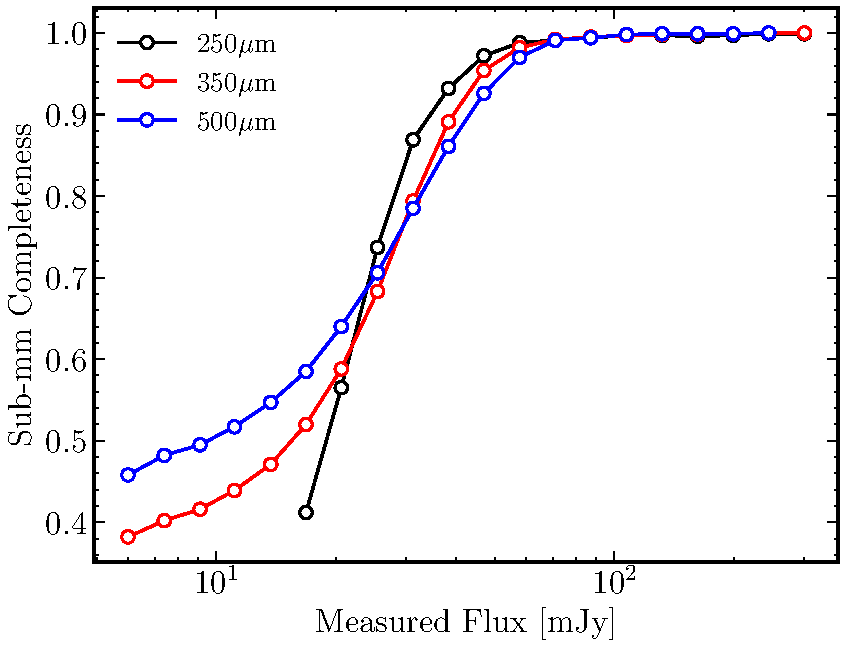
\includegraphics[width=0.8\columnwidth]{Figures/submm_completeness.pdf}
	\caption[Completeness of H-ATLAS DR1 catalogue as a function of $250\,\mu$m flux]{The completeness of the Data Release I catalogues of \textit{Herschel} sources, as a function of the measured flux density at $250\,\mu$m (black) $350\,\mu$m (red) and $500\,\mu$m (blue). This figure is recreated from Figure 21 in \citealt{Valiante_2016}.}
	\label{fig:submm_completeness}
\end{figure}

\subsection{Data Releases of the H-ATLAS}
\label{sec:Data Releases of the H-ATLAS}

The first public data release (DR1) of H-ATLAS covered the three equatorial GAMA fields, which cover approximately $25\%$ of the total survey area. These fields benefit from multiwavelength coverage from GAMA, SDSS, 2dF, the Galaxy Evolution Explorer (GALEX, \citealt{Martin_2005}), the UKIRT Infrared Deep Sky Survey -- Large Area Survey (UKIDSS-LAS, \citealt{Lawrence_2007}), the Wide-field Infrared Survery Explorer (WISE, \citealt{Wright_2010}), the VISTA Kilo-degree Infrared Galaxy survey (VIKING, \citealt{Edge_2013}) and the Kilo-Degree Survey (KiDS, \citealt{deJong_2013}). Combined across the three fields, there are a total of $113,995$, $46,209$ and $11,011$ sources detected at $> 4\sigma$ at $250$, $350$ and $500\,\mu$m, and $4,650$ and $5,685$ sources detected at $> 3\sigma$ at $100$ and $160\,\mu$m, respectively (\citealt{Valiante_2016}). Following the release of the DR1 sources, \citealt{Bourne_2016} used the Likelihood Ratio method (LR; \citealt{Sutherland_1992, Ciliegi_2003}) to identify probable optical SDSS counterparts to the sources with SNR$_{250} > 4$. We shall discuss the method in detail in Section \ref{sec:The Likelihood Ratio Method}. Sources with SNR$_{250} < 4$ that were in the DR1 catalogue due to significant $350$ or $500\,\mu$m detections were omitted from the analysis of \citealt{Bourne_2016} on the basis that they have far-IR colours indicating high redshifts, and are more likely to be misidentifed due to the increased probability of chance aligments or the effects of gravitational lensing along the line of sight \mbox{(\citealt{Negrello_2010, Pearson_2013, Bourne_2014}).}

The second public data release (DR2) covered the NGP and SGP, that together form $\sim 75\%$ of the total survey area. The NGP has coverage at optical wavelengths from the SDSS, and in the near-IR by UKIDSS-LAS. Moreover, a smaller $\sim26\,$deg$^2$ area of the field was observed by a deeper $K_s$-band survey by the H-ATLAS team using the UKIRT (with a limiting magnitude in the Vega system of $K_s = 19.40$, compared to $18.69$ for UKIDSS-LAS). The SGP is the largest field, spanning approximately half of the total H-ATLAS survey area, and has coverage from the 2dF spectroscopic survey, KiDS in four optical bands ($u$, $g$, $r$ and $i$) and VIKING in five near-infrared bands ($Z$, $Y$, $J$, $H$ and $K_s$). The DR2 \textit{Herschel} source catalogues are obtained from areas of the images that have at least two observations from the SPIRE instrument, the second pass significantly reducing the total noise at the positions of all sources, meaning that the areas covered by the catalogues are slightly smaller than the images ($177\,$deg$^2$ for the NGP and $303\,$deg$^2$ for the SGP).

The DR2 catalogues, obtained in the same manner as the first data release, contain $118,980$ sources in the NGP ($112,069$, $48,876$ and $10,368$ detected at $> 4\sigma$ at $250$, $350$ and $500\,\mu$m and $5,036$ and $7,046$ detected at $> 3\sigma$ at $100$ and $160\,\mu$m, respectively). As with DR1, short wavelength counterparts in the optical and near-IR were identified for a fraction of the \textit{Herschel} sources using the LR technique (\citealt{Furlanetto_2018}). In the SGP a preliminary counterpart identification was conducted using the Two Micron All Sky Survey (2MASS, \citealt{Skrutskie_2006}). A nearest neighbour match to within $5\,$arcsec of a 2MASS galaxy gives identifications for $3,444$ \textit{Herschel} sources, but no formal LR analysis had yet been applied. In the following section we detail the Likelihood Ratio method and apply it to the $250\,\mu$m sources detected by \textit{Herschel} in the SGP.

\subsection{The Likelihood Ratio Method}
\label{sec:The Likelihood Ratio Method}

The Likelihood Ratio method assigns a probability (\textit{reliability} in the common nomenclature) to all potential matches surrounding low resolution sources to distinguish between likely counterparts and chance alignments, and has been used many times to identify counterparts to \textit{Herschel} sources. For example, the LR method was used by \citealt{Smith_2011} to identify SDSS counterparts in the Science Demonstration Phase (SDP) catalogue; by \citealt{Kim_2012} to identify Spitzer-IRAC counterparts also in the SDP data; by \citealt{Fleuren_2012} for VIKING IDs in the Phase 1 catalogue of the GAMA9 field, and as mentioned earlier, by \citealt{Bourne_2016} and \citealt{Furlanetto_2018} to find optical and near-IR counterparts in the GAMA fields and NGP field, respectively.

The likelihood, $L$, of a counterpart being the true identification to a \textit{Herschel} source is given by the ratio between the likelihood that an object observed at a given radius from the source, $r$, with an optical or near-IR magnitude, $m$, is the true ID and the probability of observing an unassociated object with the same $r$ and $m$. On the assumption that the distance from the source and the optical/near-IR magnitude are independent of each other for the true dust emitting galaxy, we find that

\begin{equation}
\label{eq:likelihood_ratio}
    L = \frac{P(\textrm{ID}, r, m)}{P(\textrm{unassociated}, r, m)} = \frac{P(\textrm{ID}, r) P(\textrm{ID}, m)}{P(\textrm{unassociated}, r, m)}.
\end{equation}

Each term in the above equation can be defined in the following way: $f(r) \equiv P(\textrm{ID}, r)$, $q(m) \equiv P(\textrm{ID}, m)$ and $n(m) \equiv P(\textrm{unassociated}, r, m)$, where $f(r)$ represents the radial probability distribution function of positional errors between the source and counterpart, $q(m)$ represents the magnitude probability distribution of true counterparts and $n(m)$ is the magnitude distribution of background objects. By using Baye's theorem and the theorem of total probability, we can define the probability that a counterpart is the true ID given it has observed properties $r$ and $m$ as

\begin{equation}
\label{eq:reliability_one_counterpart}
    R \equiv P(\textrm{ID}| r, m) = \frac{L}{L+1}.
\end{equation}

Equation \ref{eq:reliability_one_counterpart} assumes that there is only a single candidate with a likelihood $L$, from which we can estimate the reliability that it is the true ID, $R$. For a source with multiple possible candidates, the reliability $R_j$ of the $j^{th}$ potential candidate is given by

\begin{equation}
    \label{eq:reliability_multiple_counterparts}
        R_j = \frac{L_j}{\sum_i L_i + (1-Q)},
\end{equation}

\noindent where we sum over the $L$ values for the $i$ number of counterparts found within the given search radius. The $Q$ parameter represents the fraction of all true counterparts that are brighter than the limiting magnitude of the optical/near-IR survey. This means that the introduction of the ($1 - Q$) term represents the probability that the counterpart is not observed and accounts for the fact that not all counterparts will be detected in the optical/near-IR survey. The value of $Q$ depends on the depth of the survey and the choice of passband used. In the following sections we outline the methods used to estimate the functions $f(r)$, $q(m)$ and $n(m)$, as well as the value of $Q$, required to calculate the reliability for each near-IR candidate observed on the VIKING images of the SGP.

\section{Applying the LR Method to VIKING Galaxies in the SGP Field}
\subsection{VISTA VIKING Counterparts}
\label{sec:star_galaxy_classifier}

The Visible and Infrared Survey Telescope for Astronomy (VISTA) is a $4\,$m wide field telescope located at the ESO Paranal Observatory in Chile. The telescope has five near-IR broad band filters, $Z$, $Y$, $J$, $H$ and $K_s$, that have central wavelengths between $0.88$ and $2.15\,\mu$m (\citealt{Emerson_2010}). The VIKING survey was a public survey with VISTA, covering approximately $1,500\,$deg$^2$ of sky, including an overlap of more than $360\,$deg$^2$ with the H-ATLAS survey in the GAMA and SGP fields, to a $5\sigma$ depth of $23.1$, $22.3$, $22.1$, $21.5$ and $21.2$ (AB system, \citealt{Edge_2013}) in the above five filters, respectively. The coverage from near-IR bands of VIKING are particularly useful in tracing evolved stars in local SGP galaxies, and hence their total stellar contents. This is compared to optical bands that are typically dominated by young stellar populations and more strongly affected by dust extinction (\citealt{Cole_2001}; see Figure \ref{fig:interstellar_medium}).

In our LR analysis we take all objects catalogued in the fourth data release of VIKING that have positions within $15\,$arcsec of a $250\,\mu$m \textit{Herschel} source. The previous analysis in the GAMA9 field by \citealt{Fleuren_2012} recovered $51\%$ of all $250\,\mu$m sources with a reliable VIKING $K_s$-band counterpart (we define \textit{reliable} as having a reliability, $R > 0.8$, which we shall justify later). From this, we might expect to find a similar fraction of our sources to have reliably matched near-IR counterparts. Given that the SGP field contains $193,527$ \textit{Herschel} sources, we might expect to locate the galaxies responsible for the dust emission in $\sim 100,000$ cases.

First, however, we note that a significant number of the $1,008,098$ sources in the VIKING survey are stars that would otherwise be erroneously matched to \textit{Herschel} sources if retained in our object catalogue. The far-IR/sub-mm emission emanating from these stars is most likely from debris discs or dust in outflows. To separate the stars from the extragalactic sources we use an adapted method of the star-galaxy classifier in \citealt{Baldry_2010} and apply the LR method separately for the two classes. The method of \citealt{Baldry_2010} uses near-IR $J$ and $K_s$ and optical $g$ and $i$ bands to define a line of separation between stars and galaxies in $J - K_s$ against $g - i$ colour-colour space, and is used by \citealt{Bourne_2016} and \citealt{Furlanetto_2018} to separate stellar and extragalactic objects in SDSS. Without coverage from SDSS in the SGP, we use the fourth data release of KiDS to determine optical $g$ and $i$ bands. We are able to define $g - i$ colours for $529,147$ ($52\%$) objects with a maximum separation from the VIKING position of $0.5\,$arcsec.

In the first step, we classified as stellar any object in our catalogue with \texttt{pStar} > 0.95. This parameter gives the probability that the source is a star, based on a shape parameter provided as part of the VIKING data release. This has the unintended consequence of cutting out some extragalactic point sources, such as quasi-stellar objects (QSOs), but this is outweighed by the confidence this gives us in removing stellar contaminants. This immediately classifies $51,508$ objects as stars. Next, we consider the $J - K_s$ against $g - i$ colour-colour space and define a stellar locus by converting the locus in \citealt{Baldry_2010} to the Vega system assuming $J_{\textrm{Vega}}$ = $J_{\textrm{AB}} - 0.91$ and $K_{s,\textrm{Vega}}$ = $K_{s,\textrm{AB}} - 1.85$:

\begin{equation}
    f_{\textrm{locus}} = 
    \begin{cases*}
        0.228 & $g-i$ < 0.3 \\
        0.05 + 0.615(g-i) - 0.13(g-i)^2 & 0.3 $\leq$ $g-i$ < 2.3 \\
        0.7768 & $g-i$ $\geq$ 2.3.
    \end{cases*}
\label{eq:stellar_locus}
\end{equation}

We defined the line of separation between stars and galaxies as $+0.2$ offset in $J - K_s$ from the stellar locus. The distribution of VIKING objects, the stellar locus and the separation line are illustrated in Figure \ref{fig:star_galaxy_classification}. This line of separation classifies a further $411,463$ sources ($299,525$ extragalactic and $111,938$ stellar). The remaining objects do not have matches in KiDS and thus do not have $g$ and $i$-band magnitudes. However, based on the separation line defined above, it can be seen that those objects with $J - K_s < 0.42$ will always fall in the stellar region regardless of their optical colour, and similarly, any object with  $J - K_s > 0.98$ will always lie above this line in the extragalactic region. The cross contamination of stars above the line and galaxies below the line is small, so next we defined all the remaining sources with $J$ and $K_s$ -band magnitudes using the above single colour cuts. This classified a further $102,540$ sources ($102,265$ as galaxies and $275$ as stars). Finally, we returned to the \texttt{pStar} parameter and relaxed the criteria to \texttt{pStar} > 0.7, with all remaining objects failing this being classified as galaxies. At the end of this classification system we identify $793,331$ ($78.9\%$) extragalactic sources and $212,028$ ($21.1\%$) stars.

\begin{figure}
    \centering
	\includegraphics[width=0.8\columnwidth]{Figures/star_galaxy_classification.pdf}
	\caption[$J - K_s$ against $g-i$ colour-colour plot for VIKING objects in the SGP]{The $J - K_s$ against $g-i$ colour-colour diagram of VIKING objects with KiDS identifications in the SGP. The stellar locus defined by Equation \ref{eq:stellar_locus} is illustrated as the solid blue line, while the separation between stars and galaxies, defined as $+0.2$ offset from the stellar locus, is shown as a dashed blue line. Extragalactic and stellar sources identified from our classification are shown as grey and red points respectively.}
	\label{fig:star_galaxy_classification}
\end{figure}

\subsection{Distribution of True Counterparts, q(m)}
\label{sec:true_counterparts_distribution}

To estimate the reliability of each VIKING source being the true ID, we first need to determine the probability distribution of true counterparts as a function of $K_s$-band magnitude, $q(m)$. To do this, we use the method described in \citealt{Ciliegi_2003}. First, we define the magnitude distribution of near-IR objects, separately for stars and galaxies, which we shall denote as $n'_{\textrm{total}}(m)$. Here we have set prime notation to reference raw counts, while no prime notation is reserved for counts that have been normalized to the total area searched on the VIKING images. 

Statistically speaking, if we build a magnitude distribution of all background objects, and subtract this from the observed distribution, $n'_{\textrm{total}}(m)$, we might expect this to follow the magnitude distribution of the true identifications. This excess of objects is calculated by subtracting the magnitude distribution estimated from a set of $844,715$ random positions. A total of $2,917,214$ VIKING objects were identified within $15\,$arcsec of these randomly drawn positions to form our $n'_{\textrm{background}}(m)$ (top panel of Figure \ref{fig:true_counterparts_distribution}), thus the \textit{real} counterparts has a distribution that may be expected to follow

\begin{equation}
    n'_{\textrm{real}}(m) = n'_{\textrm{total}}(m) - n'_{\textrm{background}}(m) \frac{N_{\textrm{250\,\micron}}}{N_{\textrm{background}}},
\label{eq:real_distribution}
\end{equation}

\noindent where we have scaled to the search area by $N_{\textrm{250\,\micron}}$ and $N_{\textrm{background}}$, the number of $250\,\mu$m positions in the SGP catalogue and the number of randomly located positions, respectively.

Next, we derive $q(m)$ by normalizing $n'_{\textrm{real}}(m)$ and scaling by the fraction of all true counterparts that would be visible on the VIKING images, $Q$ (see Section \ref{sec:estimating_Q}). This ensures that the integral of $q(m)$ over all magnitudes, up to the limiting magnitude of the VIKING survey, is equal to the probability that the sources is detected, i.e. $\int^{m_{\textrm{lim}}} q(m)dm = Q$. This normalization can be written as

\begin{equation}
\label{eq:true_counterparts_distribution}
    q(m) = \frac{n'_{\textrm{real}}(m)}{\sum_{m_i}n'_{\textrm{real}}(m_i)}\times Q,
\end{equation}

\noindent where we have summed over the magnitude bins, $m_i$. Our function $q(m)$ is illustrated in the middle panel of Figure \ref{fig:true_counterparts_distribution} and shows the difference between the extragalactic and stellar sources, requiring us to implement the LR method separately for the two classes. We also show in Figure \ref{fig:true_counterparts_distribution} the magnitude distributions of $n_{\textrm{total}}(m)$, $n_{\textrm{background}}(m)$ and $q(m)/n_{\textrm{background}}(m)$. 

We note that the $q(m)$ function depends on the value of $Q$, much like the reliability in Equation \ref{eq:reliability_multiple_counterparts}. To proceed further, we must be able to determine the fraction of true IDs that are observed on the VIKING images.

\begin{figure}
    \centering
	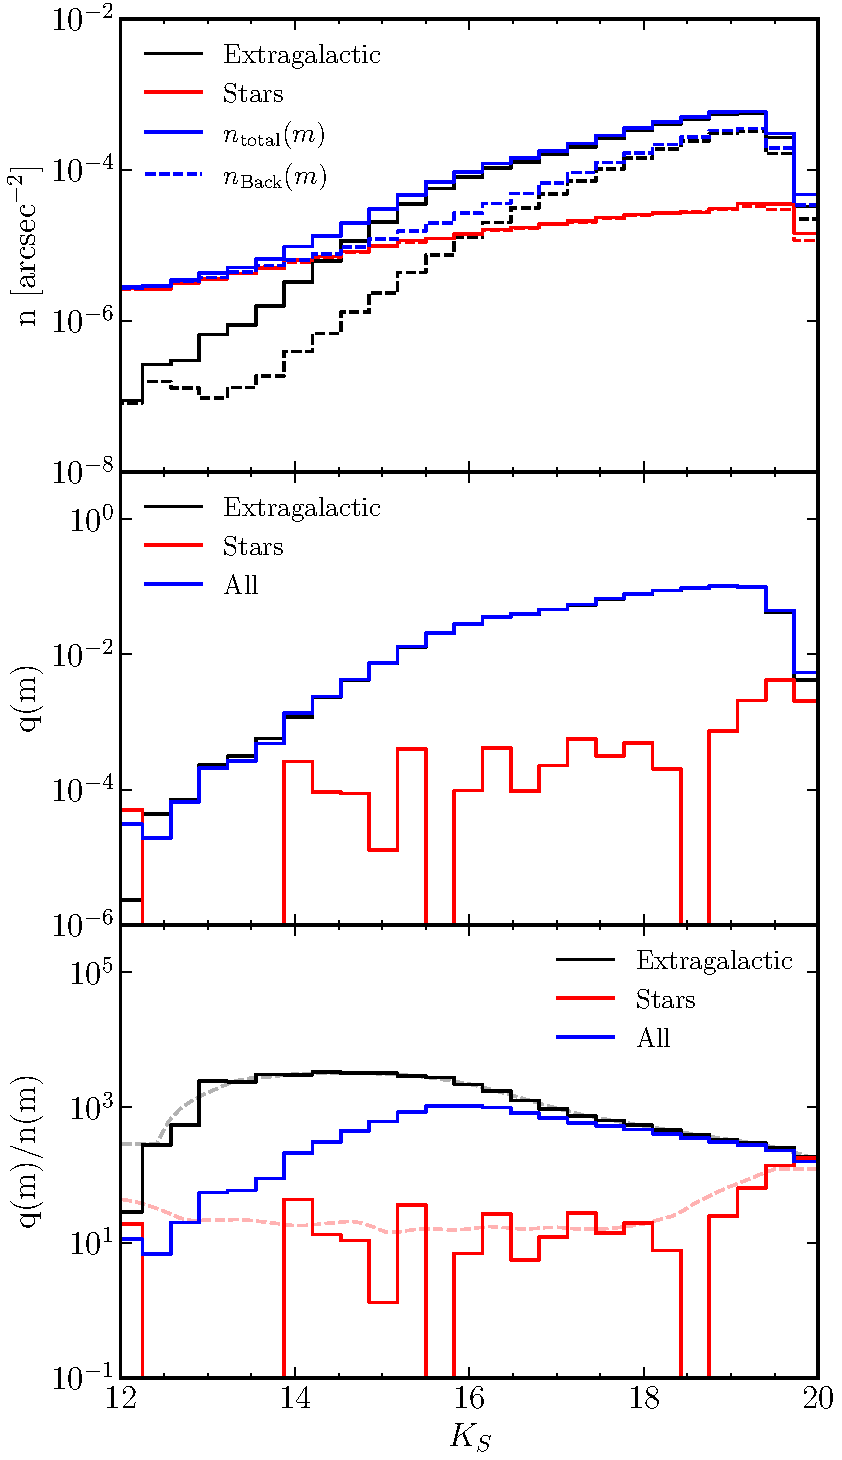
\includegraphics[height=0.75\textheight]{Figures/true_counterparts_distribution.pdf}
	\caption[$K_s$-band distribution of counterparts, separated into galaxies and stars]{Top panel: The $K_s$-band magnitude distributions of objects located within $15\,$arcsec of $250\,\mu$m \textit{Herschel} positions (blue solid line) and random positions (blue dashed line). Each histogram is separated by their extragalactic (black lines) and stellar (red lines) classification. Middle panel: The $K_s$-band magnitude distribution of \textit{true} counterparts accounting for the excess of VIKING sources observed near \textit{Herschel} sources. Bottom panel: The ratio between the \textit{true} counterparts distribution (middle panel) and the background distribution of sources, as used in the calculation of the likelihood ratios in Equation \ref{eq:likelihood_ratio}. The dashed lines represent smoothed fits to $q(m)/n(m)$ to provide a continuous function at all magnitudes. The colour convention of the middle and bottom panels are the same as the top panel.}
	\label{fig:true_counterparts_distribution}
\end{figure}

\subsection{Estimating Q}
\label{sec:estimating_Q}

We predict the probability of finding a genuine counterpart on the VIKING images below the limiting magnitude of the near-IR survey, $Q$, using the method described in \citealt{Fleuren_2012}. While some methods in the literature derive $Q$ directly by summing the $n_{\textrm{real}}(m)$ distribution and dividing by the number of SPIRE sources, this leads to a systematic overestimate due to the possibility of clustering or multiple true counterparts due to source blending. An alternative method by \citealt{Fleuren_2012} calculates an estimate of 1-$Q_0$, the probability of \textit{not} observing a VIKING counterpart, by counting the number of \textit{Herschel} sources without VIKING associations within a given search radius, $r$. These sources will be given the name \textit{blanks}, and has a dependency on search radius, $B(r)$.

Blank sources may be observed in one of several scenarios. Given that the number of cross identifications is limited not by the \textit{Herschel} survey flux limit, but on the depth of the near-IR survey, the most likely reason for observing a blank is that the real ID is fainter than the limiting $K_s$-band magnitude. However, we may also observe a blank if the counterpart lies outside the search radius or if the source is a spurious SPIRE detection.

Even when a \textit{Herschel} source has a candidate on the VIKING images, we may not definitively say that a source is not a blank as we may encounter chance alignments with other near-IR objects close to the same line of sight. Thus, to estimate the true number of blanks, we are reminded that the number of blanks we observe must also account for those that are spuriously identified as not blank. In other words, the number of observed blanks is the number of true blanks minus the number of true blanks that happen to have random VIKING interlopers. If we define the number of observed blanks as $B_{\textrm{obs}}$, the number of true blanks as $B_{\textrm{t}}$ and the number of random interlopers as $N_{\textrm{rand}}$, then

\begin{equation}
    B_{\textrm{obs}} = B_{\textrm{t}} - N_{\textrm{rand}} = B_{\textrm{t}} - B_{\textrm{t}} \times f_{\textrm{rand}},
    \label{eq:observed_blanks}
\end{equation}

\noindent where we have assumed that the number of random interlopers can be estimated from the fraction of positions that have random interlopers, $f_{\textrm{rand}}$. This fraction can itself be estimated from the set of random positions used above to calculate $q(m)$. Using a similar set of notation as before: $B_{\textrm{background}}$ to represent the number of blanks from the catalogue of random positions; $N_{\textrm{background}}$ to represent the total number of random positions and $B'_{\textrm{background}}$ representing the number of random positions for which we observe at least one VIKING counterpart (or \textit{non-blank}), we can estimate $f_{\textrm{rand}}$ as

\begin{equation}
    f_{\textrm{rand}} = \frac{B'_{\textrm{background}}}{N_{\textrm{background}}} = \frac{N_{\textrm{background}} - B_{\textrm{background}}}{N_{\textrm{background}}} = 1 - \frac{B_{\textrm{background}}}{N_{\textrm{background}}}.
\end{equation}

To scale this fraction to the size of the SGP catalogue, the same number of random positions are used as there are \textit{Herschel} $250\,\mu$m positions, such that $f_{\textrm{rand}}$ may be written as

\begin{equation}
    f_{\textrm{rand}} = 1 - \frac{B_{\textrm{background}}}{N_{\textrm{250\,\micron}}}.
\end{equation}

From substitution into Equation \ref{eq:observed_blanks}, we define the fraction of \textit{Herschel} sources that are true blanks (i.e. $B_{\textrm{t}}/N_{\textrm{250\,\micron}}$) as

\begin{equation}
    \frac{B_{\textrm{t}}}{N_{\textrm{250\,\micron}}} = \frac{B_{\textrm{obs}}}{B_{\textrm{background}}}.
    \label{eq:true_blanks}
\end{equation}

In summary, to estimate $1-Q$, we need only to divide the number of observed blank $250\,\mu$m positions by the number of observed blank random positions. It is clear that any estimate of $Q$ using this method depends on the given search radius from the \textit{Herschel} source, $r$, thus we calculate this fraction for a range of radii between $0$ and $15\,$arcsec and model the dependence of $B(r) \equiv 1 - Q$ on the search radius in the same manner as \citealt{Fleuren_2012}.

A \textit{Herschel} source that has no VIKING association within a radius $r$ is either a source whose true counterpart is too faint to be detected by the VIKING survey or lies outside the radius, or both. Assuming that such situations are independent of each other, then the probability of either occurring is given by the conditional probability:

\begin{equation}
\label{eq:blank_probability}
    P(\textrm{Blank}) = P(\textrm{Faint} \cup \textrm{Outside}) = P(\textrm{Faint}) + P(\textrm{Outside}) - P(\textrm{Faint} \cap \textrm{Outside}).
\end{equation}

The first term, the probability that the counterpart is too faint to be detected, is given by $1-Q$, while the probability that the counterpart resides outside the search radius is dependent on the probability distribution of offsets between the counterpart and \textit{Herschel} source, $f(r)$. We assume that the sources in the \textit{Herschel}-ATLAS are point-like on the $250\,\mu$m images and that the errors are equal in RA and declination for radial symmetry. While $f(r)$ naturally depends on the positional errors in both the \textit{Herschel} and near-IR detections, we can assume that the near-IR positional errors are negligible compared to those of SPIRE given that the $1\sigma$ VIKING positional errors are $< 0.2\,$arcsec (\citealt{Fleuren_2012}). For this reason, we use a radially symmetric Gaussian for $f(r)$ with width $\sigma_\textrm{pos}$ corresponding to the typical SPIRE positional error. According to the theory of total probability, the probability that an observable counterpart is detected out to any search radius must equal unity, therefore 

\begin{equation}
    \int_0^\infty 2\pi r'f(r')dr' = 1,
\end{equation}

\noindent which implies that our function $f(r)$ take the form

\begin{equation}
    f(r) = \frac{1}{2\pi\sigma_\textrm{pos}^2}e^{\frac{-r^2}{2\sigma_\textrm{pos}^2}}.
\label{eq:positional_offset_distribution}
\end{equation}

If the probability of observing a counterpart within a radius $r$ is given by

\begin{equation}
    F(r) = \int_0^r 2\pi r'f(r')dr',
\end{equation}

\noindent then P(Outside) in Equation \ref{eq:blank_probability} is given by $1 - F(r)$. Upon substitution we find that the probability of observing a blank source as a function of the search radius can be modelled using the function

\begin{equation}
    B(r) = P(\textrm{Blank}) = (1-Q) + (1-F(r)) - (1-Q)(1-F(r)) = 1 - QF(r).
\label{eq:blanks_model}
\end{equation}

In Figure \ref{fig:Q_estimate} we show the number of blank \textit{Herschel} and blank random positions as a function of the search radius (open squares and circles, respectively) as well as their ratio which is our proxy for $B_{\textrm{t}}/N_{\textrm{250\,\micron}}$ (filled circles, recall Equation \ref{eq:true_blanks}). The best fitting $B(r)$ is illustrated as the black line. Using this method we measure the value of $Q$ to be $0.835\pm0.009$ when considering extragalactic and stellar near-IR sources and $Q = 0.823\pm0.009$ when stellar contaminants are removed. This tells us that for approximately $80\%$ of \textit{Herschel} sources, we observe a near-IR counterpart on the VIKING image that is directly associated with the dust emission.

\begin{figure}
    \centering
	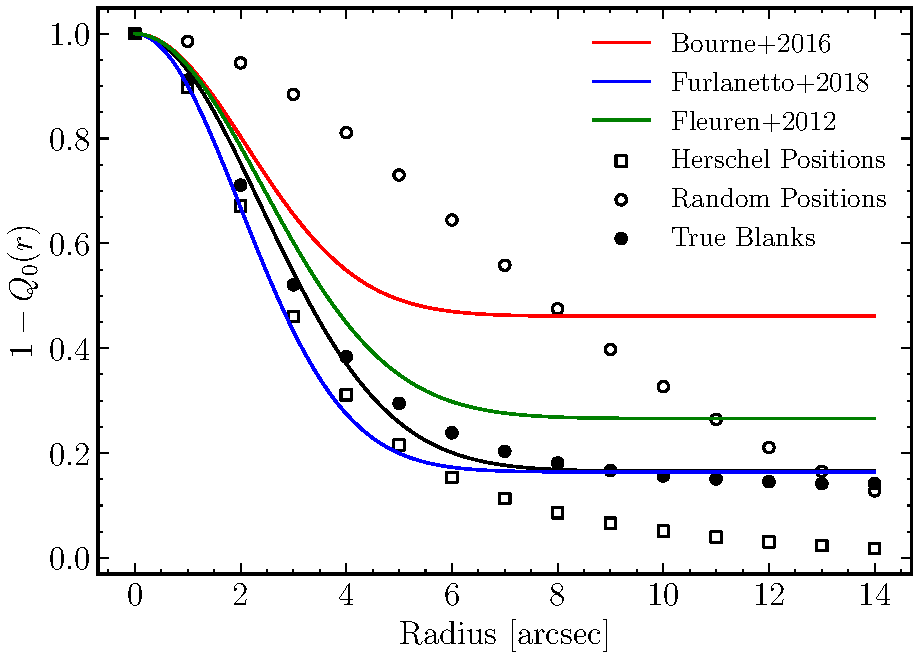
\includegraphics[width=0.67\columnwidth]{Figures/Q_estimate.pdf}
	\caption[An estimate for the number of blank sources as a function of search radius]{Estimates for the number of blanks (sources without VIKING candidates) as a function of the search radius, $r$. Open circles represent the number of blank random positions placed across the SGP field, while open squares represent the number of blank SPIRE $250\,\mu$m positions from H-ATLAS. The filled circles show the division of the two, which acts as our proxy for the fraction of SPIRE sources blank on the VIKING images. The solid black line represents the best fit to the points using Equation \ref{eq:blanks_model}. The same model used in \citealt{Fleuren_2012}, \citealt{Bourne_2016} and \citealt{Furlanetto_2018} are shown as green, red and blue lines respectively.}
	\label{fig:Q_estimate}
\end{figure}

Measurements of the value of $Q$ depend on the depth of the matching survey, and given that the near-IR is less obscured by dust than in the optical (recall Figure \ref{fig:interstellar_medium}), the $Q$ value from studies with optical $r$-band counterparts are typically lower. A comparison of the $Q$ values measured by various \textit{Herschel} studies, and the wavebands that were used, are presented in Table \ref{tab:data_release_input_surveys}.

\begin{table}
\centering
\begin{tabular}{p{3.5cm}|p{3.5cm}|p{2.5cm}|p{3.75cm}}
    \hline
    \hline
    H-ATLAS Release & Input Survey & $Q$ Estimate & Reference \\
    \hline
    \hline
    SDP & $r$ -- SDSS & $0.583$ & \citealt{Smith_2011} \\ 
    Phase 1 GAMA9 & $K_s$ -- VIKING & $0.734\pm0.026$ & \citealt{Fleuren_2012} \\
    Data Release I & $r$ -- SDSS & $0.539\pm0.001$ & \citealt{Bourne_2016} \\
    Data Release II & $r$ -- SDSS & $0.538\pm0.001$ & \citealt{Furlanetto_2018} \\
    Data Release II & $K_s$ -- UKIRT & $0.836\pm0.001$ & \citealt{Furlanetto_2018} \\
    Data Release III & $K_s$ -- VIKING & $0.835\pm0.009$ & This work \\
    \hline
\end{tabular}
\caption[Comparison of optical/near-IR surveys used in H-ATLAS studies]{Comparison of the measured values of $Q$ from \textit{Herschel}-ATLAS studies. From left to right the columns contain: the data release of H-ATLAS; the input survey and the passband used; the fraction of sources with associated counterparts observed on the optical/near-IR images, $Q$; and the reference of the study.}
\label{tab:data_release_input_surveys}
\end{table}

\subsection{Positional Uncertainty of H-ATLAS Detections}

We see from Figure \ref{fig:Q_estimate} that $B(r)$ becomes flat at approximately $3\sigma_{\textrm{pos}}$, suggesting that few counterparts are to be found at search radii greater than $\sim 7\,$arcsec. The function $B(r)$ also provides a prediction for the standard SPIRE positional error, $\sigma_{\textrm{pos}}$, which defines the width of the positional offset distribution $f(r)$. We measure this value to be $\sigma_{\textrm{pos}} = 2.388\pm0.065\,$arcsec. The positional uncertainty has a dependency on the SNR of the far-IR detection (\citealt{Bourne_2016}) and, in theory, should depend on both the full-width at half-maximum (FWHM) of the beam and the SNR following

\begin{equation}
    \sigma_{\textrm{pos}} = 0.6\times\frac{\textrm{FWHM}}{\textrm{SNR}},
\label{eq:positional_uncertainty_theory}
\end{equation}

\noindent as derived in \citealt{Ivison_2007}, on the assumption of uncorrelated noise. However, the addition of confusion noise and clustering of sources have the effect of increasing the prefactor of $0.6$ (\citealt{Chapin_2011}; \citealt{Bourne_2014}). To account for this, a scaling factor (typically about $1.09$, corresponding to a redefined prefactor of $\sim 0.65$) is often applied and is more suitable for sources extracted from far-IR/sub-mm images. To estimate the reliability of each individual counterpart, we require knowing the $1\sigma$ positional uncertainty of each $250\,\mu$m source. To do this, we first make a check on the appropriate prefactor to use in Equation \ref{eq:positional_uncertainty_theory}. Assuming a FWHM of $18\,$arcsec and the fitted value of $\sigma_{\textrm{pos}} = 2.388\,$arcsec, we use the SNR of all $250\,\mu$m sources to obtain a set of values for the prefactor. The median value of this distribution is $0.66$, which we shall use herein. Substituting the prefactor for $0.66$, we estimate $\sigma_{\textrm{pos}}$ for each \textit{Herschel} source, and thus an individual function of $f(r)$ to use when calculating the reliability values.

\section{Likelihood Ratio Results}
\label{sec:lr_results}

We apply Equation \ref{eq:reliability_multiple_counterparts} to all potential near-IR counterparts within $15\,$arcsec of a \textit{Herschel} source. As mentioned previously, the SGP catalogue contains $193,527$ far-IR sources, of which $190,788$ have at least one possible counterpart identified within our search radius. Having matched each source with its highest reliability counterpart we find that $181,373$ ($95.1\%$) are sources with VIKING identifications indicating the source is a galaxy and $9,415$ ($4.9\%$) have stellar classifications. 

In keeping with previous studies, we define reliable matches as those sources with counterparts having $R \geq 0.8$. This provides a balance between minimizing the number of falsely identified counterparts, and ensuring that the sample is not severely contaminated by blended sources. We further justify this choice later in this Section. We identified $111,065$ reliable near-IR counterparts, representing $58.2\%$ of all SGP sources for which there was at least one possible candidate. Of the reliable IDs, $110,374$ ($99.4\%$) are classified as galaxies and $691$ ($0.6\%$) as stellar. The fraction of galaxies is much higher for our reliable sample than it is for the whole VIKING catalogue (Section \ref{sec:star_galaxy_classifier}), suggesting that the LR method is highly biased against stars, as is intended. 

On the assumption that a source that is erroneously matched with a counterpart has a probability of $1 - R$, we can estimate the false ID rate for our reliable matches from

\begin{equation}
    N_{\textrm{False}} = \sum_{R_i \geq 0.8} (1 - R_i) = 5,343.
\label{eq:false_ids}
\end{equation}

We predict that there are $5,343$ \textit{false reliable} IDs in the SGP, representing $4.8\%$ of the reliable sample. This can be compared to values of 4.7\% in the GAMA fields and the NGP ($r$-band SDSS matching), 4.5\% for the NGP ($K_s$-band matching) and 4.2\% during the SDP. While the false identification rate for the SGP is in keeping with the other studies, it is the highest value. We might expect that the near-IR analyses would have the lowest false identification rates, as the limiting $K_s$-band magnitude of the VIKING survey corresponds to higher redshift galaxies than the limiting $r$-band magnitude in the SDSS studies. As mentioned earlier, the limiting factor in the number of matches we obtain is in the limits of the optical/near-IR catalogue, not the far-IR survey. This leaves many \textit{Herschel} sources at high redshift that do not get matched to any counterpart, or possibly, erroneously matched to a much lower redshift counterpart. This problem would be greater for the optical surveys, and thus they would have a higher false ID rate. However, in our analysis of the SGP, we chose to use an increased search radius of $15\,$arcsec (compared to $10\,$arcsec in other H-ATLAS studies). We chose the larger radius to avoid missing any unusual VIKING associations, such as those that might lie at larger $r$ due to the effects of gravitational lensing. As shown in \citealt{Bakx_2020}, there are still genuine associations observed on the VIKING images beyond $10\,$arcsec, and we wish to retain these in our catalogue despite them being unlikely to have significant reliability values. The result is that the average number of potential candidates increases per source, and given that the LR method requires that the sum of all candidates' reliabilities add to one, the average reliability of the true ID will fall, leading to a higher false identification rate. Further discussion on the effect of increasing the search radius is made in Section \ref{sec:multiplicity}.

The completeness, $\eta$, of the reliable sample is defined as the fraction of \textit{Herschel} sources that are recovered with a reliability greater than $0.8$ (\citealt{Smith_2011}) and can be calculated as

\begin{equation}
    \eta = \frac{n(R \geq 0.8)}{n(\textrm{SNR}_{250} \geq 4) \times Q},
\label{eq:completeness}
\end{equation}

\noindent where the numerator is the size of the reliable sample and the denominator predicts the true number of sources. As would be expected, a value of $\eta = 1$ would imply that the fraction of all counterparts deemed reliable has reached its theoretical maximum, $Q$. Another important test of our sample is the cleanness, $C$, an estimate of the number of sources that are not spurious matches, given by

\begin{equation}
    C = 1 - \frac{N_{\textrm{False}}}{N_{\textrm{250\,\micron}}}.
\label{eq:cleanness}
\end{equation}

At a minimum reliability cut of $0.8$, we find that the completeness of the reliable galaxy sample is $\eta = 78\%$, which is similar to the completeness values found for the NGP and GAMA fields of $74\%$ and $73\%$, respectively. Figure \ref{fig:completeness_and_cleanness} shows how the completeness and cleanness change for a range of different reliability thresholds. We see that a cut at $R \geq 0.8$ selects a highly clean sample at a minor expense in completeness. While an increase in the reliability cut would yield a marginally cleaner sample, it would be offset drastically by a fall in completeness. A decrease in the minimum reliability would lead to an increase in completeness, with only a small decrease in cleanness, but reducing the threshold too far would also lead to problems securing a one-to-one matching between \textit{Herschel} sources and counterparts. At $R \geq 0.8$ we set a minimum value that is a good balance between the two values.

\begin{figure}
    \centering
	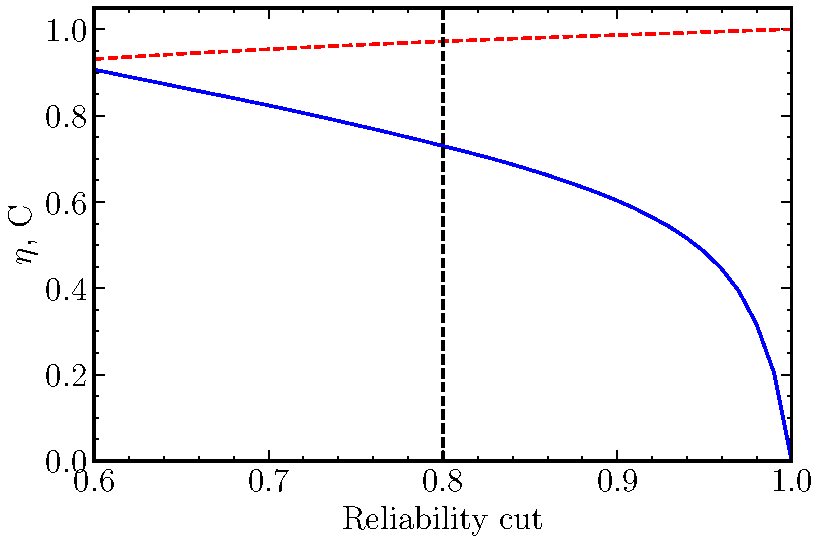
\includegraphics[width=0.8\columnwidth]{Figures/completeness_and_cleanness.pdf}
	\caption[Completeness and cleanness of the SGP sample as a function of reliabilty]{The completeness, $\eta$, and cleanness, $C$, of the SGP sample as a function of various minimum reliability values, illustrated as solid blue and red dashed lines, respectively. The vertical dashed line reprents the minimum reliability cut used in all H-ATLAS studies ($R \geq 0.8$).}
	\label{fig:completeness_and_cleanness}
\end{figure}

\section{Multiplicity of Counterparts}
\label{sec:multiplicity}

One disadvantage of using the LR method to identify counterparts to low resolution sources is that it assumes a one-to-one matching of source and counterpart. Given that the sum of reliabilities of all possible counterparts may not exceed one, we have a bias against \textit{Herschel} sources with many candidates, the result of merging galaxies, members of groups and clusters, and non-physical associations such as confusion due to blending. The combined reliabilities of multiple systems reduces the maximum reliability of the single chosen ID. For example, consider two galaxies in a cluster that are both observed on the VIKING images close to the \textit{Herschel} position. It is reasonable to imagine that these two objects may have similar $K_s$-band magnitudes and radial offsets and, if they are close to the position of the far-IR emission, may both have high likelihoods. In such a case, either source may be considered the true ID to the source (and in reality both are likely associated), but the use of Equation \ref{eq:reliability_multiple_counterparts} to measure their reliabilities leads to the following, 

\begin{equation}
    R_j \sim \frac{L_j}{\sum_i L_i} \sim \frac{L_j}{2L_j} \sim 0.5.
\end{equation}

In this scenario, neither counterpart would be considered the true ID and thus we generate a bias against multiple systems in our catalogue. Table \ref{tab:multiplicity} shows the fraction of \textit{Herschel} sources that have reliable identifications, which decreases as a function of the number of possible counterparts. This would suggest that the sample is partly incomplete because we miss sources where there are more than one genuine association on the VIKING image. In Figure \ref{fig:multiplicity} we show this reliable fraction as a function of multiplicity compared with previous H-ATLAS studies. Compared to the Science Demonstration Phase (\citealt{Fleuren_2012}), GAMA fields (\citealt{Bourne_2016}) and the NGP (\citealt{Furlanetto_2018}), we see that the SGP reliability fraction declines more slowly, peaks at higher average $N_{\textrm{Match}}$ and is slightly lower for sources where there is only a single possible counterpart. All these differences may be explained by the increased search radius. The increase from $10\,$arcsec to $15\,$arcsec is a significant change as it equates to more than double the total area of the near-IR image ($A_{\textrm{SGP}}/A_{\textrm{Other}} = \pi r_{\textrm{SGP}}^2/\pi r_{\textrm{Other}}^2 = 225\pi/100\pi = 2.25$). While the increased $r$ means that we are more likely to observe a reliable counterpart, it also increases the probability of matching erroneously with a background galaxy, thus the low fraction at $N_{\textrm{Match}} = 1$ may be due to an increase in unassociated VIKING objects being selected as the true identification. In Table \ref{tab:multiplicity} we see that the average offset between the VIKING galaxy and \textit{Herschel} source is substantially higher when the galaxy is the only possible candidate, suggesting that some fraction of these sources are erroneously matched. Occasionally, our chosen reliable ID will be unassociated with the \textit{Herschel} source, but selected for being the only observed counterpart. This is more likely to happen when there is only one candidate (and in reality the source is blank on the near-IR image), resulting in the jump in the average separation. Another reason why the reliable fraction is low for $N_{\textrm{Match}} = 1$ is that a large fraction of the stellar candidates will fall in this bin as stars tend to be isolated (\citealt{Bourne_2016}). The shift in the peak is likely due to the greater ability to discern between true IDs and background interlopers when $N_{\textrm{Match}}$ candidates are spread over double the area.

\begin{table}
    \centering
    \begin{tabular}{p{2cm}|p{2cm}|p{2cm}|p{2cm}|p{4cm}}
        \hline
        \hline
        $N_{\textrm{Match}}$ & $N_{\textrm{SPIRE}}$ & $N_{\textrm{Reliable}}$ & Percent & Av. Separation [arcsec] \\
        \hline
        \hline
        0 & 2,739 & 0 & 0 & 0 \\
        1 & 11,692 & 5,477 & 47 & 6.3 \\
        2 & 24,268 & 14,568 & 60 & 4.7 \\
        3 & 32,948 & 20,396 & 62 & 4.1 \\
        4 & 33,526 & 20,383 & 61 & 3.8 \\
        5 & 27,745 & 16,359 & 59 & 3.6 \\
        6 & 20,236 & 11,563 & 57 & 3.4 \\
        7 & 12,999 & 7,155 & 55 & 3.4 \\
        8 & 8,079 & 4,355 & 54 & 3.3 \\
        9 & 4,983 & 2,640 & 53 & 3.4 \\
        10 & 3,017 & 1,643 & 54 & 3.3 \\
        \hline
    \end{tabular}
    \caption[Reliable fraction of SGP sources as a function of the number of candidates]{The reliable fraction as a function of the number of candidates observed per source. From left to right the columns contain: the number of observed candidates per source; the number of \textit{Herschel} sources that have $N_{\textrm{Match}}$ candidates; the number of those sources whose best counterpart has a reliability greater than $0.8$; the reliable fraction given as a percentage; and the average separation between the chosen ID and the \textit{Herschel} source in arcsec.}
    \label{tab:multiplicity}
\end{table}

\begin{figure}
    \centering
    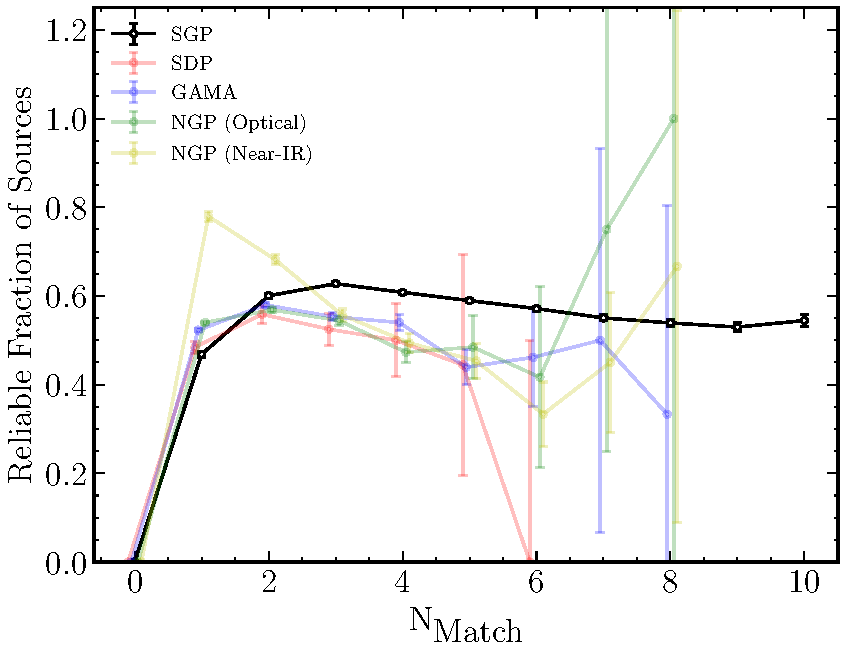
\includegraphics[width=0.67\columnwidth]{Figures/multiplicity.pdf}
    \caption[Reliable fraction of sources as a function of the number of candidates]{The fraction of \textit{Herschel} sources with reliably matched counterparts as a function of the number of observed candidates. The results from various H-ATLAS studies are shown with the following lines: SGP (black, this work), SDP (red, \citealt{Smith_2011}), GAMA (blue, \citealt{Bourne_2016}) and NGP (optical in green and near-IR in yellow, \citealt{Furlanetto_2018}). All other works used a maximum search radius of $10\,$arcsec while the SGP analysis used $15\,$arcsec. For clarity each line has been offset in $N_{\textrm{Match}}$ by a different value.}
    \label{fig:multiplicity}
\end{figure}

One way we can predict the number of \textit{Herschel} sources that are missed by the LR method due to multiple genuine counterparts, is by assuming that all candidates are true associations if their combined reliability is greater than $0.8$, but where no individual object reaches this threshold. However, in our case of large $r$, even moderately valued $R$ counterparts will combine to exceed this minimum reliability. Alternatively, we may consider the likelihood values of each counterpart, which, unlike their reliability values, do not have an upper bound. From Equation \ref{eq:reliability_multiple_counterparts} we see that a reliability of $0.8$ or greater corresponds to $L > 0.66$, assuming a single candidate and a value of $Q = 0.835$. An alternative estimate for the number of lost sources can then be made assuming that a source with a matched counterpart with $L > 0.66$ but $R < 0.8$ is likely influenced by nearby candidates. We find $33,967$ \textit{Herschel} sources that satisfy these conditions. We expect that this number is still overestimated, however, as it will include chance alignments. A more realistic number of sources with two or more physically associated counterparts requires knowing their redshifts.

As shown in \citealt{Fleuren_2012}, chance alignments along the line of sight can be ruled out by comparing the redshifts of the VIKING galaxies. They propose that associated galaxies have photometric redshifts within $\sim 10\%$ of each other, while spectroscopic redshifts fall within $\sim 5\%$. Other than catastrophic redshifts, the only other scenario in which this method fails is if the \textit{Herschel} source lies on a similar line of sight to unrelated groups or merging galaxies. In the following, we describe a new method for estimating the number of missed \textit{Herschel} sources that compares the redshifts of our VIKING counterparts with the redshifts of background galaxies. The photometric redshifts that are used in this section are described in detail in Section \ref{sec:phot_z_VIKING}.

Firstly, we restrict both the SGP near-IR counterpart catalogue and the background catalogue (from Section \ref{sec:true_counterparts_distribution}) to contain only sources with two or more counterparts. We then restrict this further to counterparts found within $8\,$arcsec of the source (or random) position. This second selection reduces the samples to likelihood ratios above $\sim 0.66$, reducing the chance of observing unrelated galaxies. For all source positions we identify the pair of galaxies with the closest redshifts and measure the quantity $\Delta z/\sigma_{\Delta z}$, the difference in redshift divided by the error in their separation. In Figure \ref{fig:delta_z_multiplicity} we show the probability distribution functions (PDFs) of $\Delta z/\sigma_{\Delta z}$ for the SGP catalogue (red line) and the background catalogue (black line). A subtraction of the latter from the former gives an excess close to $\Delta z = 0$ (blue line). The area of this peak represents the probability that a close pair of VIKING galaxies are indeed related to the \textit{Herschel} source. We fit a Gaussian profile to this excess and estimate this probability to be $2 - 5\%$. After multiplying this probability by the number of \textit{Herschel} sources where we observe a close pair of VIKING galaxies (which we shall define as having $-0.1 < \Delta z/\sigma_{\Delta z} < 0.1$), then we find an estimate for the number of \textit{Herschel} sources with genuine multiple counterparts of $\sim 400 - 1,000$.

\begin{figure}
    \centering
    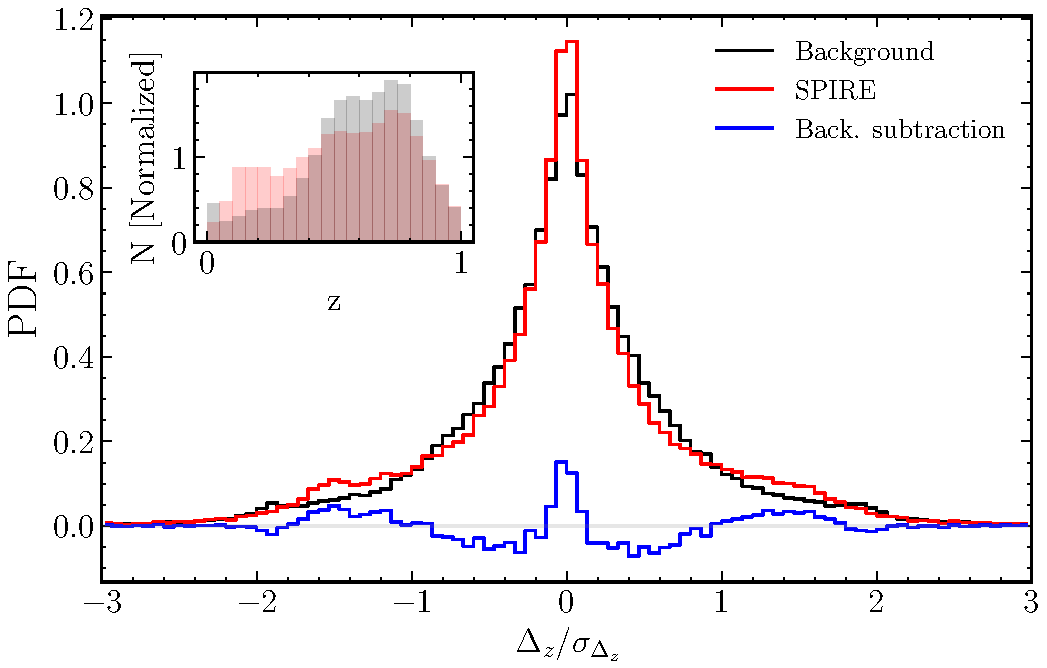
\includegraphics[width=0.8\columnwidth]{Figures/delta_z_multiplicity.pdf}
    \caption[PDFs of $\Delta z/\sigma_{\Delta z}$ for \textit{Herschel} sources and random positions]{Probability distribution functions for the quantity $\Delta z/\sigma_{\Delta z}$, the difference in photometric redshifts divided by the error on this value. This quantity is calculated for pairs of VIKING galaxies located within $8\,$arcsec of a \textit{Herschel} position (red histogram) and random positions (black histogram). The blue histogram represents a background subtraction of the former. The excess located at $\Delta z = 0$ represents the probability that a pair of VIKING counterparts with similar redshifts are associated with the \textit{Herschel} source. The inset figure shows the normalized redshift distribution of counterparts observed within $8\,$arcsec of the $250\,\mu$m positions in red and random positions in grey.}
    \label{fig:delta_z_multiplicity}
\end{figure}

It should be noted that this method is independent of the LR method, and so the closest redshift pair may not always contain the counterpart with the highest reliability. In total we observe $70,880$ sources with pairs of near-IR counterparts at similar redshifts, but only three quarters of these contain our chosen identification. The remaining quarter of sources may be located along the same line of sight as unrelated galaxy interactions, or the multiple system is related to the \textit{Herschel} source, but is overlooked by the one-to-one matching of the LR technique. The subset of sources in this method represents approximately one third of the whole SGP catalogue ($70,880/193,527$), and so we expect many more galaxy groups and mergers to be in the full SGP survey. Moreover, there is evidence to suggest that the merger rate of galaxies evolves with redshift, and peaks at $z \sim 1$ (e.g. \citealt{Bell_2006, Ryan_2008}). If true, then a large fraction of the interacting systems in the SGP may be beyond the detection limit of the VIKING survey, and are the cause of some of the blank fields.

\section{Photometric Redshifts}

\subsection{Redshifts of the \textit{Herschel} Sources}
\label{sec:phot_z_Herschel}

Any study on the evolution of the properties of galaxies requires knowing its redshift. With far-IR sources and their near-IR counterparts, we can begin to construct SEDs that constrain both the stellar and dust emission. The far-IR spectra of \textit{Herschel} galaxies are well described by a two-temperature modified blackbody model, as presented in \citealt{Pearson_2013}. This model takes the form 

\begin{equation}
    S_\nu = A[B_\nu(T_{\textrm{hot}})\nu^\beta + \alpha B_\nu(T_{\textrm{cold}})\nu^\beta],
\label{eq:pearson_sed_model}
\end{equation}

\noindent where $S_\nu$ is the flux density of the source at the rest frame frequency, $\nu$, $A$ is a normalization factor, $B(T)$ represents the Planck function at temperature $T$ (here we assume two dust temperatures, $T_{\textrm{hot}}$ and $T_{\textrm{cold}}$), $\beta$ is the dust emissivity index and $\alpha$ represents the fraction of cold dust mass to hot dust mass. Using a sample of $40$ H-ATLAS sources with spectroscopic redshifts, \citealt{Pearson_2013} found that the best fitting set of parameters were $T_{\textrm{hot}} = 46.9\,$K, $T_{\textrm{cold}} = 23.9\,$K and $\alpha = 30.1$ (assuming a fixed value of $\beta = 2$). Assuming these fixed values, we define the model given by Equation \ref{eq:pearson_sed_model} with just two free parameters, the overall normalization and the redshift of the galaxy. We use this model to determine the photometric redshifts of our galaxies directly from the dust emission. It is a useful model to apply to our SGP sample as we have few \textit{Herschel} observations with which to constrain the far-IR SED and therefore cannot use a model with many parameters. For each source the normalization and redshift were varied until the following $\chi^2$ reached a minimum:

\begin{equation}
    \chi^2 = \sum_i \frac{(S_i - S_{i,m})^2}{E_i^2}.
    \label{eq:chi_squared}
\end{equation}

$S_i$ represents the flux density at each \textit{Herschel} wavelength, $i$, $S_{i,m}$ is the model prediction of the flux and $E_i$ is the flux density error. As discussed in Section \ref{sec:Detecting Submillimeter Sources on Herschel Images}, the \textit{Herschel} sources in DR2 have flux density errors obtained from images including instrumental and confusion noise, but they do not contain a calibration error. The calibration error is formed of two parts: i) the main contribution comes from the uncertainty in imaging a set of calibration objects, which in the case of SPIRE is Neptune and for PACS is a group of stars and asteroids. This error is correlated between the bands and is approximately $4\%$ for SPIRE; and ii) a contribution uncorrelated between bands of $1.5\%$ (\citealt{Valiante_2016}). While the correlated error scales all fluxes by the same amount, and therefore does not impact on the $\chi^2$, the uncorrelated errors do contribute and are calculated by adding in quadrature the errors in the DR2 catalogue with the errors obtained by multiplying the flux density of each source by $1.5\%$ such that $\bar{E_i} = \sqrt{E_i^2 + (S_i \times 0.015)^2}$, where $\bar{E_i}$ is the new, calibration included error and replaces $E_i$ in Equation \ref{eq:chi_squared}.

The $1\sigma$ errors on our photometric redshifts were taken to be the range above and below the best-fitting value where the $\chi^2$ increases by one. When taking all sources collectively, the mean reduced $\chi^2$ ($\chi_\nu^2 = \chi^2/\nu$ where $\nu$ is the number of degrees of freedom) should have a value of $\sim 1$ if the model sufficiently represents the data. A mean value of $\chi_\nu^2 > 1$ would suggest that the model is not a good representation of the data, while a mean value $\chi_\nu^2 < 1$ implies that either the model has too many free parameters or that the errors on the data are too large. The $\chi^2$-minimization applied to the sources in the SGP yields a mean value of $\chi_\nu^2 = 0.55$. Given that the model requires only two free parameters, it is more likely that this low value is a result of overestimated flux uncertainties. While the errors on the photometric redshifts account for all relevant uncertainties in the flux densities, it does not account for uncertainty in the model SED of \citealt{Pearson_2013}, especially given that high-redshift \textit{Herschel} galaxies have been shown to have a variety of SED shapes (\citealt{Bakx_2018}). The H-ATLAS sources used to generate the characteristic SED of \citealt{Pearson_2013} are intrinsically bright (facilitating their spectroscopic redshift search) and thus have fractionally smaller errors on their flux densities than the full H-ATLAS sample. This results in errors in the photometric redshifts smaller than appropriate for the wide variety of sources observed in H-ATLAS. For this reason, the redshift error estimated by \citealt{Pearson_2013}, $\Delta z/(1+z) = 0.12$, should represent a minimum redshift error that is caused by the diversity of real galaxy SEDs, and should be taken as a minimum value when applied to the SGP data. For $\sim 9\%$ of sources the measured redshift error is lower than this minimum value and we have therefore replaced the redshift error from the SED fitting with $\Delta z/(1+z) = 0.12$. The median redshift of the \textit{Herschel} sources in the SGP is $\sim 1.4$ and has a peak at a similar value. More than $100$ \textit{Herschel} galaxies have $z > 5$. The distribution of photometric redshifts can be seen in Figure \ref{fig:redshift_distribution} in blue.

\subsection{Redshifts of the VIKING Counterparts}
\label{sec:phot_z_VIKING}

We obtain photometric redshifts for the VIKING counterparts by matching the catalogue to the \textit{Herschel} Extragalactic Legacy Project (HELP; \citealt{Vaccari_2016, Shirley_2019}). HELP provides an extensive catalogue of extragalactic sources observed across \textit{Herschel} surveys. The photometric redshifts in HELP are based on the template-fitting method of \citealt{Duncan_2018a} and the machine learning method of \citealt{Duncan_2018b}.

The approach combines the redshift posterior distributions from template fitting with those from machine learning to generate a final distribution from their Bayesian combination. Three different sets of templates were used: the default library of SEDs provided with the photometric redshift code \texttt{EAZY} (\citealt{Brammer_2008}); the XMM-COSMOS templates of \citealt{Salvato_2009} and \citealt{Salvato_2011}, which cover a wide range of galaxy spectral types including active galactic nuclei (AGN) and QSO templates; and the atlas of galaxy SEDs presented in \citealt{Brown_2014}, a set of 129 galaxy SED templates based on a range of nearby galaxies including ellipticals, spirals and luminous IR galaxies. The machine learning algorithm uses a training set compiled from a sample of $48,995$ galaxies with spectroscopic redshifts in the SGP plus further redshifts from the three GAMA fields (the surveys used in the training set include the 2dF, 6dF, 2MRS and SRSS2 surveys). Three separate redshift estimates were made using three sets of filters: $u$, $g$, $r$ and $i$ from OmegaCAM on the VLT Survey Telescope; $g$, $r$, $i$, $z$ and $y$ from the Dark Energy Camera (DECam) on the Victor M. Blanco 4-meter Telescope; and $J$ and $K_s$ from the VISTA InfraRed CAMera (VIRCAM) on VISTA, along with the aforementioned $g$, $r$ and $i$ bands from OmegaCam. The machine learning redshifts were generated using the redshift code GPz (\citealt{Almosallam_2016}). The template and machine learning derived redshift posteriors were then combined using the Hierarchical Bayesian combination method described in \citealt{Dahlen_2013} to generate a single redshift posterior for each HELP galaxy.

The redshift of the counterparts are taken from the full posterior distribution in the following way. First, an 80\% highest probability density (HPD) credible interval (CI) was calculated by starting at the peak redshift probability and lowering a threshold until 80\% of the total probability lies above the line. The resulting HPD CI may have two or more peaks, in such cases they are ranked from the most to least probable based on their peak value. The redshift is assumed to be the median of the primary peak. Next, to estimate the errors on the redshift, we assumed that the upper and lower boundaries of the primary peak defines a Gaussian, symmetric about some mean redshift close to the median redshift. We thus transform the $80\%$ credible interval into $1\sigma$ errors assuming a Gaussian distribution where an $80\%$ CI is equal to $1.282\sigma$.

In total there are $29,790,690$ objects with photometric redshifts in the HELP catalogue of the SGP field. We use a $0.5\,$arcsec matching radius to find the nearest neighbour to all the VIKING counterparts. This yields $542,302$ ($54\%$) redshifts, corresponding to $82,195$ ($74\%$) sources in our reliable SGP sample. Given the limiting magnitude of the VIKING survey, most counterparts have $z < 1$. This covers only a fraction of all \textit{Herschel} sources in the SGP, but does improve on the redshifts reached by the SDSS, which have very few galaxies beyond $z \sim 0.5$. The distribution of redshifts for the VIKING counterparts can be seen in Figure \ref{fig:redshift_distribution} in red. The median uncertainty on the counterpart redshift is $\sim 0.21$, while the far-IR sources have redshifts with uncertainties $\sim 0.51$. Thus, to derive the most accurate photometric redshift distribution of the \textit{Herschel} sources, we preferentially chose to use the redshift of the counterpart, and failing this, use the redshift estimated from \textit{Herschel} fluxes. This optimal distribution is shown in black in the same figure.

\begin{figure}
    \centering
    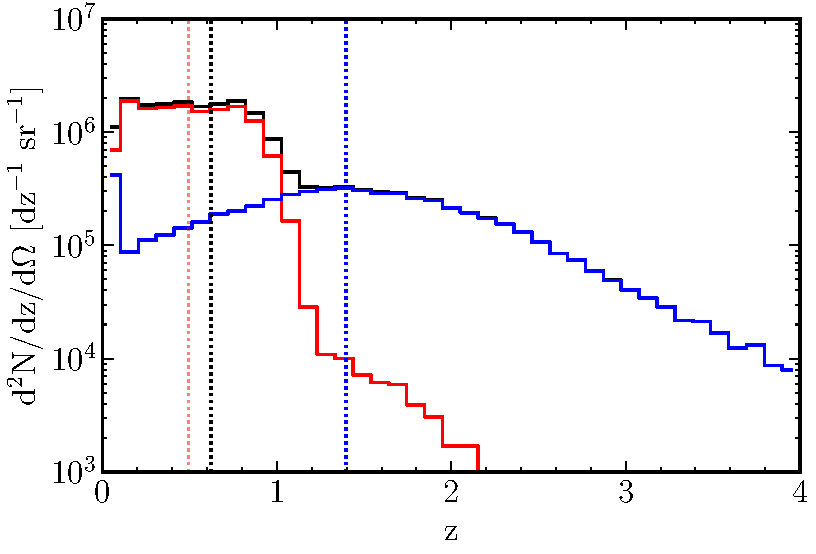
\includegraphics[width=0.8\columnwidth]{Figures/redshift_distribution.pdf}
    \caption[Photometric redshift distribution of SGP sources]{Photometric redshift distribution of the sources in the SGP field of H-ATLAS. The blue line represents the distribution of redshifts obtained from the SED fitting of the far-IR flux densities; the red line represents the distribution of redshifts for the near-infrared counterparts, as matched with the \textit{Herschel} Extragalactic Legacy Project; and the black line represents the distribution of the best estimate for each source, preferentially selecting the redshift of the counterpart. The median redshifts are $z_{\textrm{far-IR}} = 1.40$, $z_{\textrm{near-IR}} = 0.49$ and $z_{\textrm{best}} = 0.62$ and are illustrated by the dotted red, blue and black vertical lines respectively.}
    \label{fig:redshift_distribution}
\end{figure}

\section{Gravitational Lensing in the SGP}

When the light from a distant galaxy is close to the same line of sight as a foreground mass, whether that be an individual galaxy (likely a massive elliptical) or galaxy cluster, the magnification of the background source due to the deflection of the light makes the galaxy appear brighter with a larger angular size. This effect, known as gravitational lensing, makes these systems ideal targets for studying intrinsically faint and distant galaxies that may otherwise be impossible to observe. This effect can be exploited to generate a sample of prime targets for certain studies, such as investigating the physical conditions in distant star forming galaxies, measurement of the cosmological parameters (e.g. \citealt{Kochanek_1992, Kochanek_1996, Grillo_2008, Oguri_2012, Eales_2015}) and the evolution of the equation of state of dark matter (e.g. \citealt{Zhang_2009}). 

Identifying the signs of gravitational lensing (e.g. Einstein rings) from follow up imaging can be very time-consuming and not practical for large surveys. However, wide area, blank field far-IR surveys have been shown to contain a vast number of lensing events, that can be easily detected from their bright far-IR emission (e.g. \citealt{Blain_1996, Perrotta_2002, Negrello_2007, Paciga_2009, Bakx_2020}). The source counts of unlensed (by which we mean not lensed) \textit{Herschel} galaxies falls dramatically at high flux densities ($S_{500} \gtrsim 100\,$mJy), leaving a population of galaxies that are either at low redshift, bright radio galaxies, or lensed candidates. We can remove the former populations from shallow optical and radio surveys, providing a flux limited sample of far-IR sources with a high likelihood of being lensed, and low contamination. This method has been used many times in previous studies of \textit{Herschel} surveys. \citealt{Negrello_2010} produced the first sample of strongly lensed \textit{Herschel} galaxies (SLGs), presenting $5$ lensed galaxies within the SDP. This was followed by the study of \citealt{Wardlow_2013} that identified $13$ lensed galaxies from HerMES. \citealt{Nayyeri_2016} presented a further $77$ candidates from the $372\,$deg$^2$ of sky covered by the HerMES Large Mode Survey (HeLMS) and the \textit{Herschel} Stripe 82 Survey (HerS; \citealt{Viero_2014}). More recently, \citealt{Negrello_2017} identified a sample of $80$ candidates for lensing from $\sim 600\,$deg$^2$ of the H-ATLAS. In the subsequent sections we shall present a statistical sample of candidate lensed sources from the SGP, first by selecting the brightest sources using the method outlined in \citealt{Negrello_2017}, then extending this to lower flux densities by predicting the likelihood of gravitational lensing based on the redshift distributions of the far-IR sources and their near-IR counterparts. 

\subsection{The Brightest Lensed Sources}
\label{sec:brightest_lenses}

The number counts of unlensed sources falls rapidly at $500\,\mu$m flux densities above $\sim 100\,$mJy because of the steep luminosity function of far-IR selected galaxies. For a given luminosity, the probability of a galaxy having an intrinsic brightness of such high flux density becomes much lower than the probability that an intrinsically fainter source is being magnified due to gravitational lensing. Selecting all sources in the SGP with $S_{500} > 100\,$mJy we find $179$ sources, $175$ of which had at least one observed VIKING counterpart. 

The low-redshift spirals and flat spectrum radio galaxies that contaminate this sample were identified and removed by searching the location of the sources with the NASA/IPAC Extragalactic Database (NED). We also removed two variable stars (HATLASJ012658.0-323234 -- R Sculptoris and HATLASJ225519.6-293644 -- V Piscis Austrini) and five blazars, as listed in Table \ref{tab:blazars}. In total 131 local galaxies were identified from their resolved image in NED and thus removed. Their locality can be inferred from a far-IR colour-colour plot. These objects have much \textit{bluer} far-IR colours than the remaining sample (Figure \ref{fig:submm_colours_lensed_candidates}), suggesting that despite their equally high flux density, they are separate populations at different redshifts. The remaining $41$ sources with \textit{redder} colours, and thus most likely to be at high redshifts, were retained and form our bright lensing candidates. The complete sample of sources is tabulated in Appendix \ref{app:candidate_lenses_bright}. The colour-colour plot shown in Figure \ref{fig:submm_colours_lensed_candidates} illustrates how a relatively clean sample of lensed candidates (barring possible blazars) can be obtained from far-IR/sub-mm fluxes alone.

\begin{table}
    \centering
    \begin{tabular}{p{3.75cm}|p{3.25cm}|p{2cm}|p{2cm}|p{2cm}}
        \hline
        \hline
        H-ATLAS IAU Name & NED Identification & $S_{\textrm{250\,\micron}}$ [mJy] & $S_{\textrm{350\,\micron}}$ [mJy] & $S_{\textrm{500\,\micron}}$ [mJy] \\
        \hline
        \hline
        J014310.0-320056 & PKS 0140-322 & 96.0$\pm$7.5 & 119.5$\pm$8.4 & 122.4$\pm$9.0 \\
        J014503.4-273333 & [HB89] 0142-278 & 131.4$\pm$7.8 & 179.2$\pm$8.8 & 234.4$\pm$9.0 \\
        J222321.6-313701 & PKS 2220-318 & 86.0$\pm$9.5 & 110.9$\pm$10.5 & 131.9$\pm$11.7 \\
        J224838.6-323551 & [HB89] 2245-328 & 119.2$\pm$7.7 & 152.8$\pm$8.3 & 194.7$\pm$8.6 \\
        J235347.4-303746 & PKS 2351-309 & 77.1$\pm$7.4 & 96.6$\pm$8.4 & 103.1$\pm$8.9 \\
        \hline
    \end{tabular}
    \caption[Blazars in the SGP with $S_{500} > 100\,$mJy]{The blazars with $500\,\mu$m flux density $> 100\,$mJy identified in the SGP using NED.}
    \label{tab:blazars}
\end{table}

\begin{figure}
    \centering
    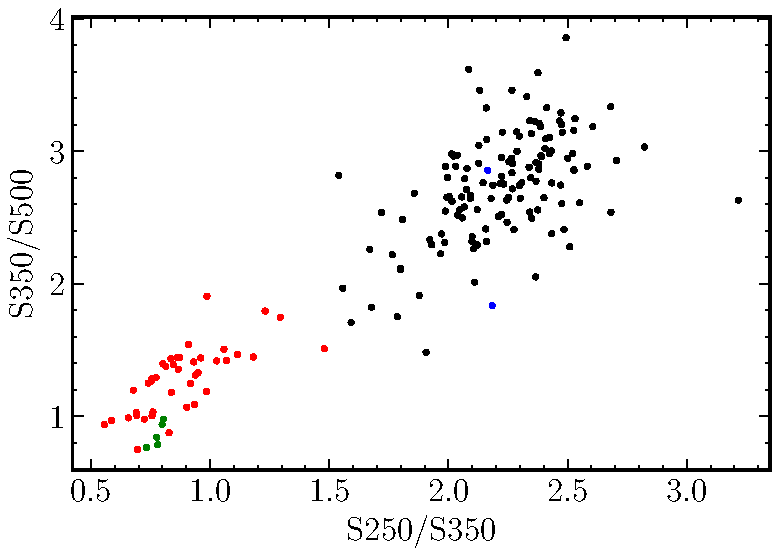
\includegraphics[width=0.8\columnwidth]{Figures/submm_colours_lensed_candidates.pdf}
    \caption[$S_{250}/S_{350}$ against $S_{350}/S_{500}$ diagram of SGP sources with $S_{500} > 100\,$mJy]{A colour-colour diagram ($S_{250}/S_{350}$ against $S_{350}/S_{500}$) for objects with $S_{500} > 100\,$mJy in the SGP. Sources are coloured according to their classification: local galaxies (black), variable stars (blue), blazars (green) and the remaining sources that we take as our candidates for lensing events (red).}
    \label{fig:submm_colours_lensed_candidates}
\end{figure}

The 41 bright candidates include $30$ that were previously identified in \citealt{Negrello_2017}. The $11$ additional sources fall outside of the mask of the SGP used in \citealt{Negrello_2017}. The mask was used to remove the edges of the survey area covered by fewer scans from the SPIRE instrument and thus were affected by higher noise. While the method described here only goes as far as to suggest that these \textit{Herschel} sources are at high redshift, at the time of publication of \citealt{Negrello_2017}, optical to near-IR imaging had only discounted one source from the initial sample for not being strongly lensed. The studies mentioned previously predict that the surface density of SLGs above $100\,$mJy at $500\,\mu$m is $\sim 0.1 - 0.2\,$deg$^{-2}$ (\citealt{Vieira_2010, Wardlow_2013, Nayyeri_2016}). Assuming that all $41$ sources in the SGP are being lensed, the surface density of lensed sources is $0.14\,$deg$^{-2}$. It is interesting to note that two sources with $S_{500} > 100\,$mJy have no VIKING counterpart within $15\,$arcsec and a further $13$ do not have photometric redshifts from HELP. These bright systems may be interesting examples of sources where the lens is at a high redshift (beyond $z \sim 1$), sources that are lensed by a cluster, or not being lensed at all.

\subsection{Extending the Search for Lenses to Lower Fluxes}

While selecting the brightest \textit{Herschel} sources is an easy and effective method for sampling those with the highest probability of lensing, the chance of a \textit{Herschel} source being lensed need not be dependent on its intrinsic brightness and many lensing events are missed because their magnification factors do not substantially lift their fluxes above the level of other, more intrinsically bright unlensed sources. An alternative way to predict the probability that a source is lensed is to compare the redshifts of the near-IR counterparts and the dust emitting source. On the assumption that the counterpart is not the true identification for the galaxy, but rather a foreground deflector, the redshift of the counterpart would be much lower than the redshift of the \textit{Herschel} galaxy.

Comparing the properties of \textit{Herschel} sources and their counterparts has already been used in previous studies to predict gravitational lensing events; a notable example of this being the Statistical \textit{Herschel}-ATLAS Lensed Objects Selection (SHALOS; \citealt{Gonzalez-Nuevo_2019}) which was used to predict that there are several hundred SLG candidates in the GAMA and NGP fields. In \citealt{Gonzalez-Nuevo_2019} these properties include their redshifts (the greater the disparity the higher the probability); the angular separation of the source and object (the closer to the same line of sight the higher the probability); the ratio between the optical and \textit{Herschel} flux densities; and the luminosity of the source compared to other galaxies at similar redshifts. For simplicity we implement a comparison of their redshifts only. The reason for this is two-fold. First, the flux density ratio and luminosity parameters require a comparison with other galaxies, which would mean that the method is not self-contained and cannot be applied to a set of low resolution sources without some prior knowledge. Secondly, the probability from the SHALOS method is higher if the angular separation between the source and counterpart is small. While this is true of galaxy-galaxy strong lensing events, the observed angular separation between \textit{Herschel} sources and optical/near-IR counterparts in \citealt{Bakx_2020} illustrate that lensing by galaxy groups or clusters may contribute significantly at lower flux densities on larger angular scales.

To provide a metric for the disparity between two probability distributions we use the Bhattacharyya coefficient. Assuming two continuous probability distributions $p_1$ and $p_2$, the Bhattacharyya coefficient is defined as

\begin{equation}
    BC(p_1, p_2) = \int \sqrt{p_1(z) p_2(z)} dz.
\end{equation}

The Bhattacharyya coefficient is closely related to the Bhattacharyya distance, $D(p_1,p_2)$, which is defined as

\begin{equation}
    D(p_1, p_2) = -\textrm{ln}[BC(p_1, p_2)].
\label{eq:Bhattacharyya_distance}
\end{equation}

Assuming that our redshift probability distributions are well described by Gaussians with means $\mu_1$ and $\mu_2$, and standard deviations $\sigma_1$ and $\sigma_2$, the Bhattacharyya distance can be simplified to

\begin{equation}
    D(p_1, p_2) = \frac{1}{4}\textrm{ln}\Bigg[\frac{1}{4}\Bigg(\frac{\sigma_1^2}{\sigma_2^2}+\frac{\sigma_2^2}{\sigma_1^2}+2\Bigg)\Bigg] + \frac{1}{4}\Bigg[\frac{(\mu_1 - \mu_2)^2}{\sigma_1^2 + \sigma_2^2}\Bigg].
\label{eq:Bhattacharyya_distance_gaussian}
\end{equation}

The final step in calculating the lensing probability of each source, $p_{\textrm{lens}}$, is to let $p_{\textrm{lens}} = 1 - BC(p_1, p_2)$, as it is through large differences in the two redshift values that we expect to observe candidates for lensing. Logically, for the VIKING galaxy to be magnifying the dust emission, the far-IR estimated redshift must be higher than the redshift of the counterpart. To ensure we are not biased by systems where the median redshift of the counterpart is higher than the source due to catastrophic photometric redshift errors, we add to the lensing probability any area of the normalized probability distribution of the sub-mm source that lies below $\mu_\textrm{near-IR} - 3\sigma_\textrm{near-IR}$. This additional term is negligible for most sources, but suppresses the probability for those sources where $z_\textrm{near-IR} > z_\textrm{far-IR}$. As such, no such contaminants are found in the SGP at lensing probabilities greater than $0.6$. Figure \ref{fig:lens_probability_scatter} shows a comparison of the near-IR and far-IR estimated redshifts. The limiting $K_s$-band magnitude and the larger errors on the source redshifts force a skewed distribution where most sources have $z_\textrm{far-IR} > z_\textrm{near-IR}$. To ensure we do not include a large number of sources in our lensed catalogue that happen to have $z_\textrm{far-IR} > z_\textrm{near-IR}$ by chance, we require a minimum lensing probability such that the difference in redshift is statistically different from the 1:1 relation.

\begin{figure}
    \centering
    \includegraphics[width=0.8\columnwidth]{Figures/Figure_2_10.pdf}
    \caption[Comparison of source and counterpart photometric redshifts]{Density plot showing a comparison between the redshifts measured from the \textit{Herschel} flux densities with the redshifts of the near-IR counterparts matched to the \textit{Herschel} Extragalactic Legacy Project. The 1:1 line is illustrated as a dashed black line and the average uncertainty in both redshift estimates is shown.}
    \label{fig:lens_probability_scatter}
\end{figure}

The rationale for our minimum lensing probability is that it should construct a sample of candidates with the fewest contaminating unlensed sources (potentially at the expense of having a smaller catalogue). While it is not possible without follow up imaging to know whether any individual \textit{Herschel} source shows signs of gravitational lensing, we can estimate this probability statistically for the whole sample. In order to do this, we predict the number of contaminants in our catalogue as a function of lensing probability, and choose the value for which this false identification rate is at a minimum. We estimate the false positive rate in two ways. First, the probability of any source, $i$, not being lensed is given by $1 - p_{\textrm{lens, i}}$, thus the sum 

\begin{equation}
N_{\textrm{not lensed, 1}} = \sum_{i}^{N_{\textrm{lenses}}}{1 - p_{\textrm{lens, i}}}
\label{eq:unlensed_estimate_1}
\end{equation} 

\noindent for all sources above some value of $p_{\textrm{lens}}$ gives one prediction for the number of spuriously selected unlensed sources that would contaminate the sample.

The second estimate comes from the fact that the Likelihood Ratio analysis leads to a false identifiation rate, where for some fraction of the \textit{Herschel} sources we match to the wrong counterpart. Earlier we estimated that $4.8\%$ of sources are spuriously matched to a VIKING counterpart. For these \textit{Herschel} galaxies there is no association between the dust emission and the near-IR counterpart. We therefore count these galaxies as spurious contaminants in our lensed catalogue if they have redshifts that are so different that they are more likely to be in the lensed sample than not. Assuming a counterpart at a redshift of $0.5$, the lowest redshift of the source before it is more likely to be classified as lensed than not is at $z \sim 2.5$. We therefore calculate our second estimate using

\begin{equation}
N_{\textrm{not lensed, 2}} = N_{\textrm{Reliable}} \times f_{\textrm{False}} \times f_{\textrm{(z > 2.5)}},
\end{equation} 

\noindent where $N_{\textrm{Reliable}}$ is the number of sources in the reliable sample, $f_{\textrm{False}}$ is the false identification rate, and $f_{\textrm{(z > 2.5)}}$ is the fraction of sources with far-IR estimated redshifts greater than $2.5$. The two methods, $N_{\textrm{not lensed, 1}}$ and $N_{\textrm{not lensed, 2}}$ are combined and divided by the total size of the lensed catalogue to define the probability of observing a false positive, P(False Positive). This is shown as a function of $p_{\textrm{lens}}$ in Figure \ref{fig:lens_false_positive}. The false positive rate has a minimum value at $p_\textrm{lens} = 0.94$, which we took to be the optimal probability threshold for gravitational lensing. At this value, the number of spuriously unlensed galaxies in the lensed sample is expected to be approximately $6\%$. Based on this minimum probability, we identify $5,923$ candidates for gravitational lensing with flux densities below $100\,$mJy at $500\,\mu$m (in Section \ref{sec:lensed_number_counts} we compare the number counts of our lensed candidates with galaxy evolution models).

\begin{figure}
    \centering
    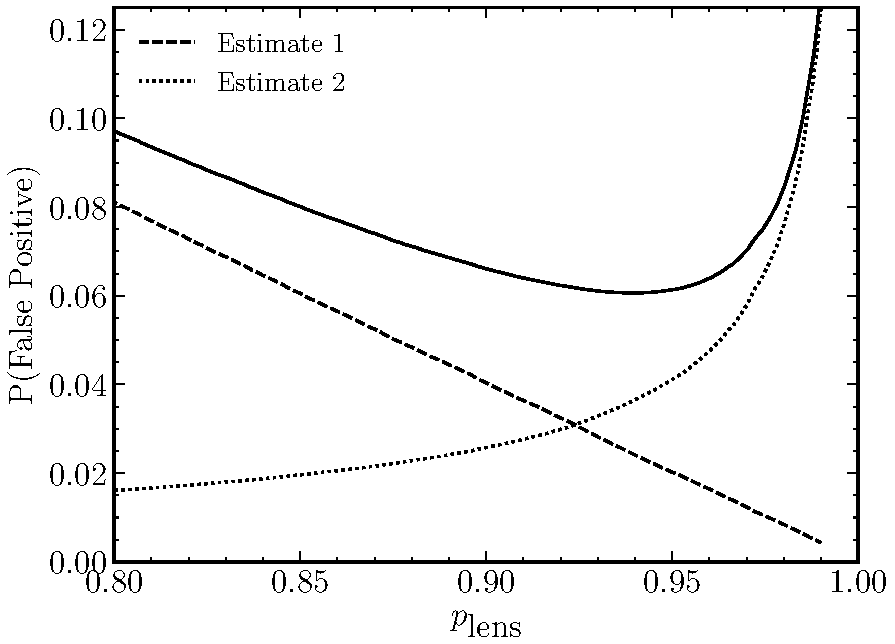
\includegraphics[width=0.62\columnwidth]{Figures/Figure_2_11.pdf}
    \caption[Fraction of unlensed sources in our lensed sample as a function of $p_\textrm{lens}$]{The false positive rate, the fraction of sources in the lensed catalogue that are unlensed, as a function of the threshold probability for gravitational lensing, $p_\textrm{lens}$. The false positive rate is split into two components: the first calculated assuming that the probability of any source, $i$, not being lensed is given by $1 - p_{\textrm{lens, i}}$ (dashed line), the second estimated from the fraction of sources in the reliable ($R > 0.8$) SGP sample that are likely to be spuriously matched to a VIKING counterpart and have a far-IR predicted redshift large enough that the \textit{Herschel} galaxy is more likely contained in the lensed catalogue than not (dotted line). The total is the combination of the two estimates (solid line).}
    \label{fig:lens_false_positive}
\end{figure}

A notable disadvantage of this method is that it relies on having matched a \textit{Herschel} source to a near-IR counterpart with high reliability. In reality, these high probability matches are the locations of galaxies where we are most confident that the near-IR galaxy is the source of the dust emission. This leads to an underestimate of the true number of lensing events. We could lower the reliability threshold for this calculation, but the false identifications rates become much more uncertain.

We also applied this method to the subset of sources with $S_{500} > 100\,$mJy. From the $41$ candidates listed in Appendix \ref{app:candidate_lenses_bright}, $24$ have near-IR counterparts with $R > 0.8$ and $19$ of these have a photometric redshift from the HELP catalogue. In most cases the probability of gravitational lensing is greater than $0.95$ and the mean probability is $0.89$. This suggests two things, one, that the bright candidates are indeed likely to be sources lensed by a VIKING foreground object, and two, that the simple method described above may be a reasonably accurate measure of lensing events in \textit{Herschel} fields for lower flux densities.

\subsection{Number Counts and Redshift Distribution of Lensed Candidates}
\label{sec:lensed_number_counts}

To assess how well our simple selection method compares to galaxy evolution models, we compare the redshift distribution and number counts of \textit{potentially} lensed \textit{Herschel} sources with the predictions from the evolution model of \citealt{Cai_2013}. When comparing the source counts from the $\sim 16\,$deg$^2$ SDP field to a selection of models, it was found that the model of \citealt{Negrello_2007} gave the closest match to observations (\citealt{Clements_2010}). Given that the work of \citealt{Cai_2013} is a development of the \citealt{Negrello_2007} model, and it also incorporates the effect of strong gravitational lensing, it should be suitable for comparison with the observations in the SGP. The galaxy evolution model of \citealt{Cai_2013} combines a physical, forward model for protospheroidal galaxies and AGN at $z \geq 1.5$ with a phenomenological backward model for late-type galaxies at $z \leq 1.5$. At these lower redshifts, the model assumes a combination of `warm' starburst galaxies and `cold' normal-type galaxies. The model also incorporates the effect of gravitational lensing on the observed source counts of these galaxies at IR wavelengths, assuming a fixed magnification value. To compare with the lensed candidates described here, we chose to use a variant of the \citealt{Cai_2013} model where the maximum magnification due to gravitational lensing is set at $\mu = 12$, a value that provides good agreement with the lensed number counts of \citealt{Negrello_2017}.

We combined together the sources with $p_{\textrm{lens}} > 0.94$ with the bright candidates from Section \ref{sec:brightest_lenses} to create a complete sample of SGP lensing candidates. In the top panel of Figure \ref{fig:lens_distributions_against_cai} we show the redshift distribution for all SGP sources (solid black line) as well as the redshift distribution of lensed sources (solid red line) and their deflectors (solid pink line). We compare these to the predictions from \citealt{Cai_2013}, which are shown using dashed lines of the same colours. The distributions show that while the total number of sources is well predicted by the model, there is a large discrepancy in the number of lensed systems at all redshifts. When illustrated as a function of the $500\,\mu$m flux density (middle panel), we see that the large disagreement in the counts of lensed sources comes from low flux densities. This discrepancy is corroborated by the lensing fraction -- the fraction of all galaxies that are likely being lensed -- shown in the bottom panel of Figure \ref{fig:lens_distributions_against_cai}. While the model of \citealt{Cai_2013} predicts that the probability of lensing is very low and approaching zero at low flux densities, the candidate lenses in the SGP continue to contribute $\sim 5 - 10\%$ of the total source counts at close to the detection limit at $500\,\mu$m.

A possible explanation for the underprediction of the number of lenses in the SGP by the \citealt{Cai_2013} model is that it is limited to strong lensing ($\mu > 2$) events, whereas our simple method relies solely on the redshifts of the galaxies and thus is not limited by their apparent brightness. Studies of the spatial cross-correlation between \textit{Herschel} galaxies in the GAMA fields and SDSS galaxies (\citealt{Gonzalez-Nuevo_2014, Gonzalez-Nuevo_2017}) have shown that the amplification of clustered galaxies by foreground structures can be explained by weak gravitational lensing ($\mu < 2$). These studies have shown that the majority of magnification bias occurs not from single galaxies, but from small groups of galaxies with one or two massive galaxies and several satellites. We may therefore ask ourselves whether our discrepancy with the \citealt{Cai_2013} model is due to the inclusion of strong and weak gravitational events, and that VIKING galaxies may act as signposts to the locations of galaxy groups.

\begin{figure}
    \centering
    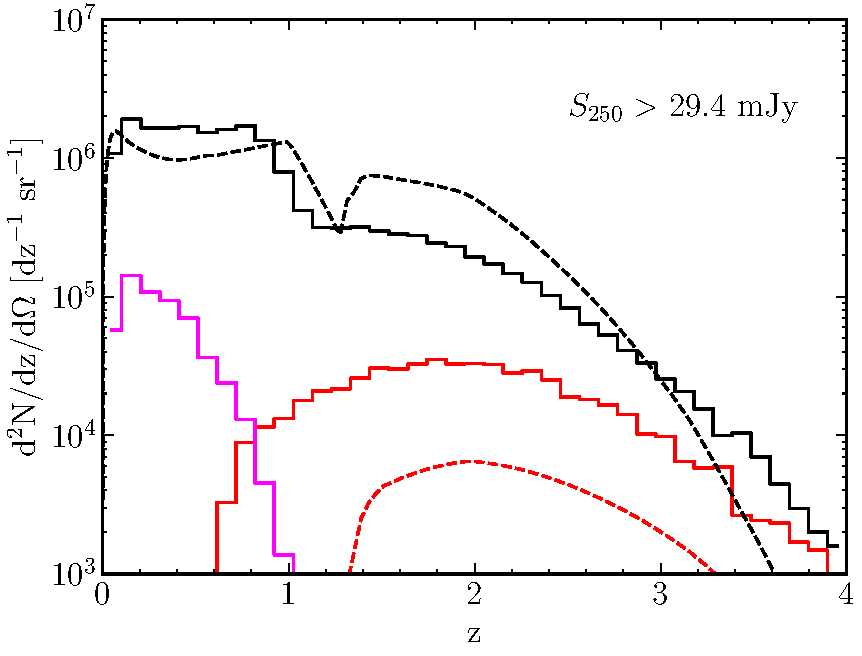
\includegraphics[width=0.55\columnwidth,height=0.255\textheight]{Figures/lens_redshift_distribution.pdf}
    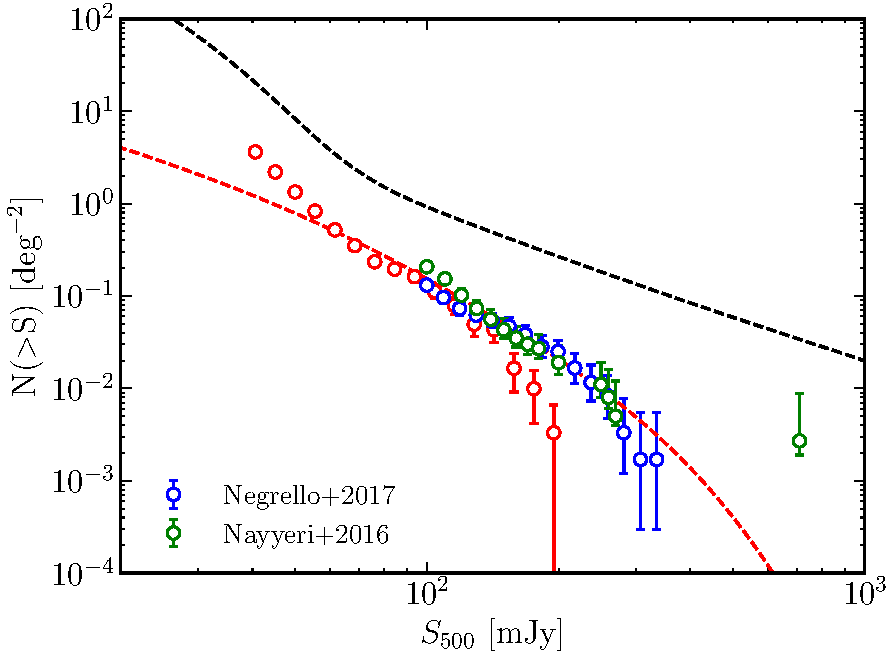
\includegraphics[width=0.55\columnwidth,height=0.255\textheight]{Figures/lens_number_counts.pdf}
    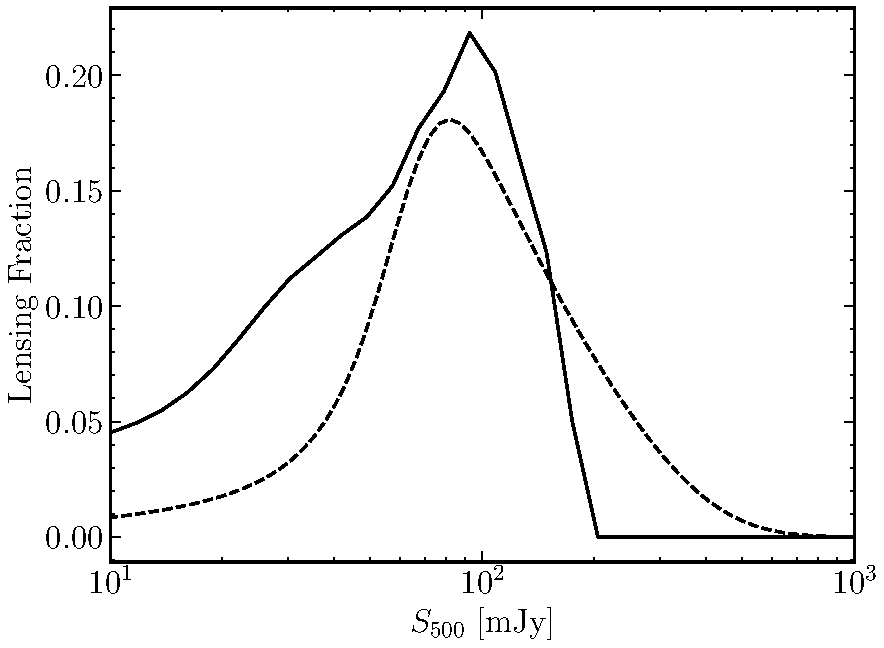
\includegraphics[width=0.55\columnwidth,height=0.255\textheight]{Figures/lensing_fraction.pdf}
    \caption[Comparison of our unlensed and lensed galaxy populations]{Top panel: The photometric redshift distribution of \textit{Herschel} sources (solid black line), as well as the distribution of lensed sources (solid red line) and their deflectors (solid pink line). The predictions from the \citealt{Cai_2013} model are shown as dashed lines using the same colours, except for the distribution of foreground deflectors which are not provided as part of the model. Middle panel: The cumulative number counts as a function of $500\,\mu$m flux density, using the same colour convention as above. The observations are now shown as error bars alongside the studies of \citealt{Nayyeri_2016} (green error bars) and \citealt{Negrello_2017} (blue error bars). Bottom panel: The fraction of sources that we predict are lensed in the SGP as a function of $500\,\mu$m flux density (solid black line), compared to the prediction from \citealt{Cai_2013} (dashed black line).
    \label{fig:lens_distributions_against_cai}}
\end{figure}

\section{Conclusions}

In this Chapter, we introduced the \textit{Herschel}-ATLAS project and implemented the Likelihood Ratio method for identifying near-IR counterparts to \textit{Herschel} sources in the South Galactic Pole field. We predicted the efficacy of the method by estimating the completeness, cleanness, and false identification rate of our sample. For $193,527$ \textit{Herschel} sources in the field, we were able to reliably match $110,374$ ($57\%$) with a VISTA VIKING counterpart, to greater than $80\%$ confidence. The completeness of the sample is $78\%$ and the false identification rate is expected to be approximately $5\%$. The data products for the H-ATLAS project are now complete\footnote{The H-ATLAS project can be found at https://www.h-atlas.org.}. In total, the survey detected over $400,000$ sources at $250\,\mu$m over $660\,$deg$^2$, with approximately half of these being matched with high significance to an optical or near-IR object. As a result, the $100,000$ newly identified far-IR bright galaxies presented here represent a doubling in the size of the H-ATLAS catalogue with reliable IDs. We showed from the similarity in the photometric redshifts of counterparts that there are likely to be between $400$ and $1,000$ sources in the SGP field that are the result of multiple VIKING galaxies. Finally, we searched for gravitational lensing events and observed $41$ bright candidates (with $500\,\mu$m flux densities greater than $100\,$mJy) and presented a method that predicts a further $\sim 6,000$ strong and weak lensing events that could be observed at lower flux densities. In the following Chapter, we shall estimate some fundamental properties of the interstellar dust in these galaxies, and from them, estimate the dust content in galaxies over cosmic time.
